% !TEX root = ../main.tex

% 预习报告	
\setcounter{section}{0}
\section{APL1-3 氦氖激光综合实验\\ Preview Report}


%---------------------------------------------------------------------
% 实验目的
\subsection{Purpose}
\begin{enumerate}
	\item 理解激光谐振原理,掌握激光谐振腔的调节方法,学会测量激光光斑功率大小;
	\item 了解激光器的纵模与横模的区别,掌握测量和改变激光器纵模的方法;
	\item 理解激光光束特性的主要参数,掌握激光传播特性的主要参数的测量方法;
	\item 了解激光光束变换的原理,掌握对高斯光束的变换与测量。
\end{enumerate}


%---------------------------------------------------------------------
% 仪器用具
\subsection{Instruments \& Equipment}

The experimental instruments and equipment are shown in the \cref{tab:Instruments}.

\begin{table}[htbp]
	\centering
	\caption{氦氖激光综合实验室实验用具}
	\label{tab:Instruments}
	\begin{tabular}{|c|m{6cm}|m{8cm}|c|}
		\hline
		\textbf{编号} & \textbf{仪器用具名称} & \textbf{主要参数(型号、规格等)} & \textbf{数量} \\ \hline
		1 & 法布里-珀罗干涉仪 & 波长 633nm,精细系数大于100,3.75G & 1 \\ \hline
		2 & 氦氖内腔激光器 & 633nm, P>1.5mW, TEM$_{00}$ & 1 \\ \hline
		3 & 氦氖半外腔激光管 & 半外腔 250 激光管,含 3 个腔片 & 1 \\ \hline
		4 & 氦氖半外腔激光器 & 半外腔, 633nm, >1.5mW, TEM$_{00}$ & 1 \\ \hline
		5 & 激光功率计 & 100nW-100mW 测试范围 & 1 \\ \hline
		6 & CMOS 相机 & 120 万像素,黑白,1292×964,3.75µm 像素,1/3 & 1 \\ \hline
		7 & 钢尺 & 500mm & 1 \\ \hline
		8 & 激光器电源部件 & & 1 \\ \hline
		9 & 白屏(带刻度) & 外形 210×150×2mm,单面带一维刻度 & 1 \\ \hline
		10 & 窗口 & $\Phi$25.4mm, T=2mm, 0.2\% 透过率,装在转接座中 & 1 \\ \hline
		11 & 窗口 & $\Phi$25.4mm, T=2mm, 10\% 透过率,装在转接座中 & 1 \\ \hline
		12 & 窗口 & $\Phi$25.4mm, T=2mm, 2\% 透过率,装在转接座中 & 1 \\ \hline
		13 & 窗口 & $\Phi$25.4mm, T=4mm, 装在相机转接座中 & 1 \\ \hline
		14 & 可变光阑 & 通光 $\Phi$2-$\Phi$28mm,外径 $\Phi$50mm & 1 \\ \hline
		15 & 平凸透镜 & $\Phi$25.4mm, f=75mm,装在 F2.5 透镜/反射镜座中 & 1 \\ \hline
		16 & 双凸透镜 & $\Phi$40mm, f=150mm,装在 F4.0 透镜/反射镜座中 & 1 \\ \hline
		17 & 相机转接座 & 装 $\Phi$25.4mm 镜片,C 接口 & 1 \\ \hline
		18 & 转接座 & 装 $\Phi$25.4mm 镜片 & 1 \\ \hline
		19 & 十字叉丝板 & 90×70×2mm,中心 $\Phi$1mm 小孔 & 1 \\ \hline
		20 & 干板夹 & 外形 60×26×24mm & 1 \\ \hline
		21 & 相机转接底板 & 转接水星相机与支杆 & 1 \\ \hline
		22 & 90mm 导轨 & 90mm 宽, 30mm 高, 1200mm 长 & 2 \\ \hline
		23 & 90mm 滑块 & 120mm 宽, 40mm 长 & 2 \\ \hline
		24 & 90mm Y 向移动滑块 & 120mm 宽, 40mm 长, Y 轴平移 & 2 \\ \hline
		25 & 调节套筒 & L76mm & 6 \\ \hline
	\end{tabular}
\end{table}


%---------------------------------------------------------------------
% 原理概述
\subsection{Principle}
\begin{enumerate}
	\item 激光和激光器的基本概念
	\begin{itemize}
		\item “激光”一词代表“\textbf{受激辐射光放大}”(Light Amplification by Stimulated Emission of Radiation)。   激光是通过\textbf{吸收辐射能量}而放大的光。激光辐射由\textbf{激光源}生成,高密度能量激发晶体棒(固态激光)或特殊气体混合物(气体激光)而产生激光辐射。此能量以光线(闪光灯光或二极管激光器)或以电释放的形式(相当于荧光灯)提供。水晶棒或激光激活气体位于两个镜子之间,形成\textbf{激光谐振腔},将激光引向特定方向,通过此方式放大光信号。激光以确定比例部分穿过透光镜,用于材料加工。
		
		激光具有三个主要特性:
		\begin{itemize}
			\item \textbf{单一性}:激光辐射只包含一种特定波长的光;
			\item \textbf{相干性}:相位一致;
			\item \textbf{平行性}:激光光束内的光高度平行。
		\end{itemize}
		激光通过聚焦透镜前是高度平行的。在激光束焦距内,会产生极高能量强度,可用于熔化或蒸发材料。此外,使用合适的光学元件(镜片),可以引导和反射激光,而且即便远距离也不会出现任何损耗。定位系统(激光笔)或振镜扫描仪用作移动式系统。由于激光束不会钝化,因此这是一种通用、无磨损工具。
		
		\item \textbf{激光的原理简介:}
		
		原子(分子)从外部吸收能量后,从下准位(低能级状态)跃迁至上准位(高能级状态)。这种状态被称为受激状态。受激状态是一种不稳定的状态,将会很快返回至低能级状态。这一行为被称为“\textbf{跃迁}”。跃迁又可分为三种形式﹕
		\begin{itemize}
			\item \textbf{吸收}:外部光线进入时,原子内的电子吸收光后从最低的能量状态(基态)进入高能状态。 随着能量增加,电子从正常轨道转移到外层轨道。 这种能量增加的状态叫做”受激“。
			\item \textbf{自然发射}:受激的电子,在所吸收能量的作用下,能级上升。 经过一定的弛张期后,能级上升的电子想要稳定下来,所以释放能量以回到较低的能量状态。 此时,能量以含有相同能量的光的形式被释放。这种现象叫做”自然发射“。
			\item \textbf{受激发射}:高能状态下存在的电子,在所持能量以相同能量的光发射时,发射的光具有完全相同的能量,相位和运动方向。换言之,发射时的一个光子变成了两个光子。 这种现象称为”受激发射“。 受激发射产生的光具有相同的能量,相位和运动方向。 因此,利用受激发射产生的大量光线在以上三个元素设定一致时能产生强烈的光线。
		\end{itemize}
		\textbf{激光基本上就是由第三种跃迁机制所产生的。}
		
		要利用自然发射振荡激光束,就必须将高能状态的电子增加到对低能量状态电子具有压倒性优势的密度。 这种现象称为”\textbf{粒子数反转状态}“。换言之,当自然发射光的量超过吸收光时,就能首次有效地产生激光束。在粒子数反转状态中,当一个电子自然发光时,该光线会使不同的电子自然发光。这样产生的连锁反应会增加光量并产生强光束。 这就是\textbf{激光振荡}的工作原理。
		
		\item 所有激光器都包含以下三个组件:
		\begin{itemize}
			\item \textbf{泵浦源}:泵浦源将\textbf{外源能量供给}激光器。
			\item \textbf{受激介质(增益介质)}:受激介质位于激光器内部,取决于不同的激光器结构设计,激光介质可能是气体混合物 (CO2 激光)、晶体棒 (YAG 固体激光) 或 玻璃纤维 (光纤激光)。\textbf{激光介质在获得外部泵浦源的能量供给时,受激产生能量辐射。}
			\item \textbf{谐振腔}:被激发的介质位于谐振腔两端两个镜子的中间位置,其中一个镜子是\textbf{单向透镜}(半反镜),受激介质产生的能量辐射在谐振腔内放大,与此同时,\textbf{只有一种特定的辐射光能够穿过单向透镜,形成一束辐射光},这一辐射光束即是激光。
		\end{itemize}
		
		\begin{figure}[h]
			\centering
			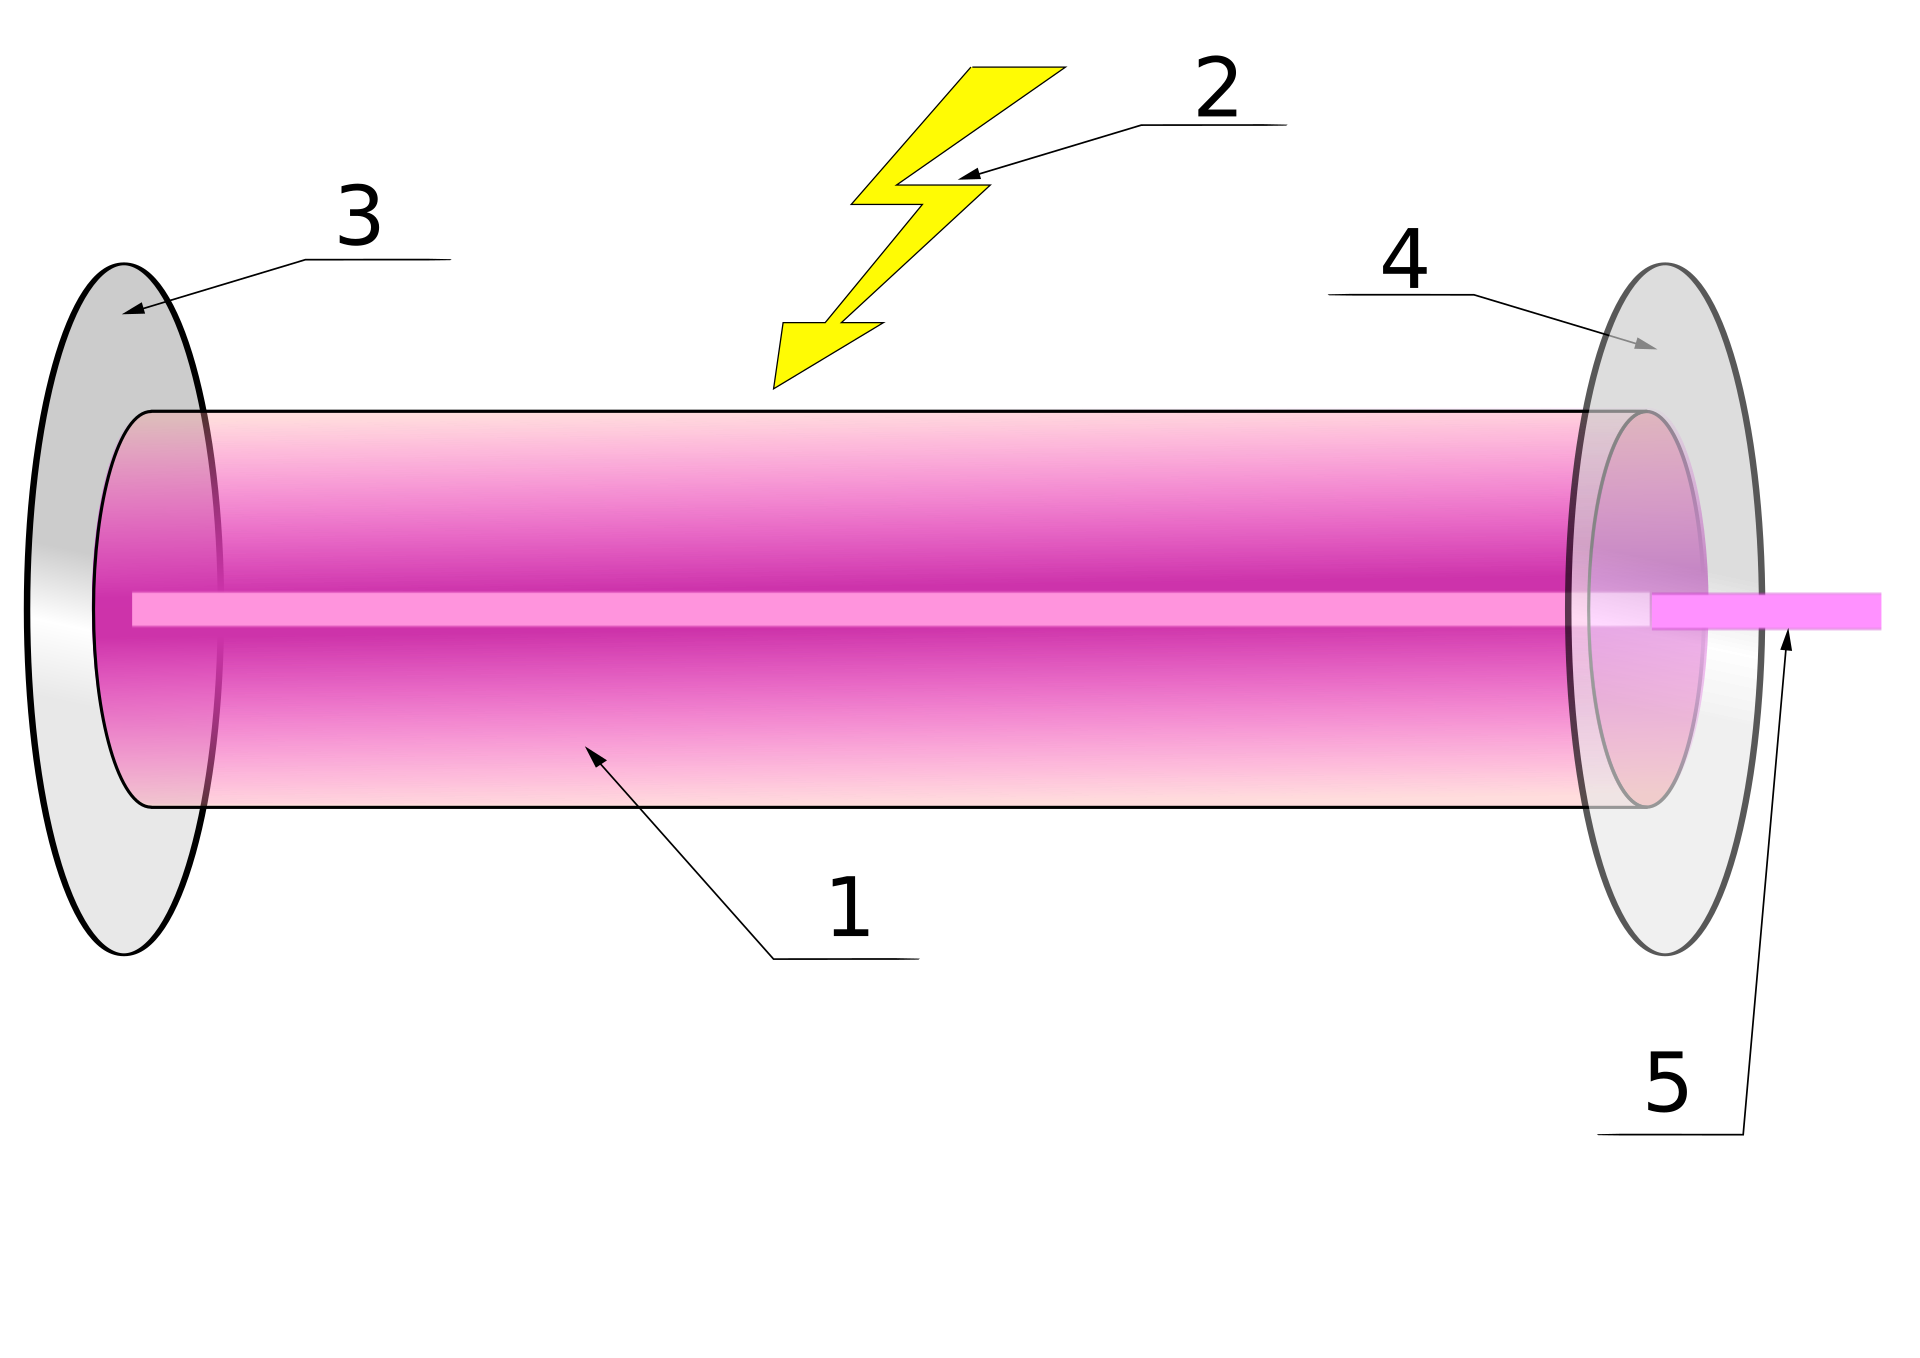
\includegraphics[width=0.5\linewidth]{APL1_8_Laser_structure.png}
			\caption{典型激光器的组成:1增益介质、2激光泵浦能量、3高反射镜、4输出耦合器、5激光束(\cite{a})}
			\label{fig:apl18laserstructure}
		\end{figure}
		
		\item \textbf{氦氖激光器}:
		\begin{itemize}
			\item 氦氖激光器是研制成功的第一种气体激光器,由激光放电管、谐震腔和激励
			电源三部份组成。其工作原理是以\textbf{四能级}方式工作的,\textbf{产生激光的是氖原子},氦
			原子只是把它吸收的能量共振转移给氖原子,起很好的媒介作用。\textbf{当氦氖原子气
			体在放电管中时,通过电子碰撞的激发,氦原子由基态跃迁到亚稳态能级,处于
			这一能级的原子与氖原子碰撞时,将能量传递给氖原子,使其向不同的能态跃迁,
			从而产生不同波长的激光}。也是最常用的一种,通常在可见光频段(632.8nm)工作。
			功率一般约数毫瓦,连续发光。因为制造方便、较便宜、可靠,所以使用较多。
			由于单色性好,相干长度可达数十米以致数百米。
			\begin{figure}[h]
				\centering
				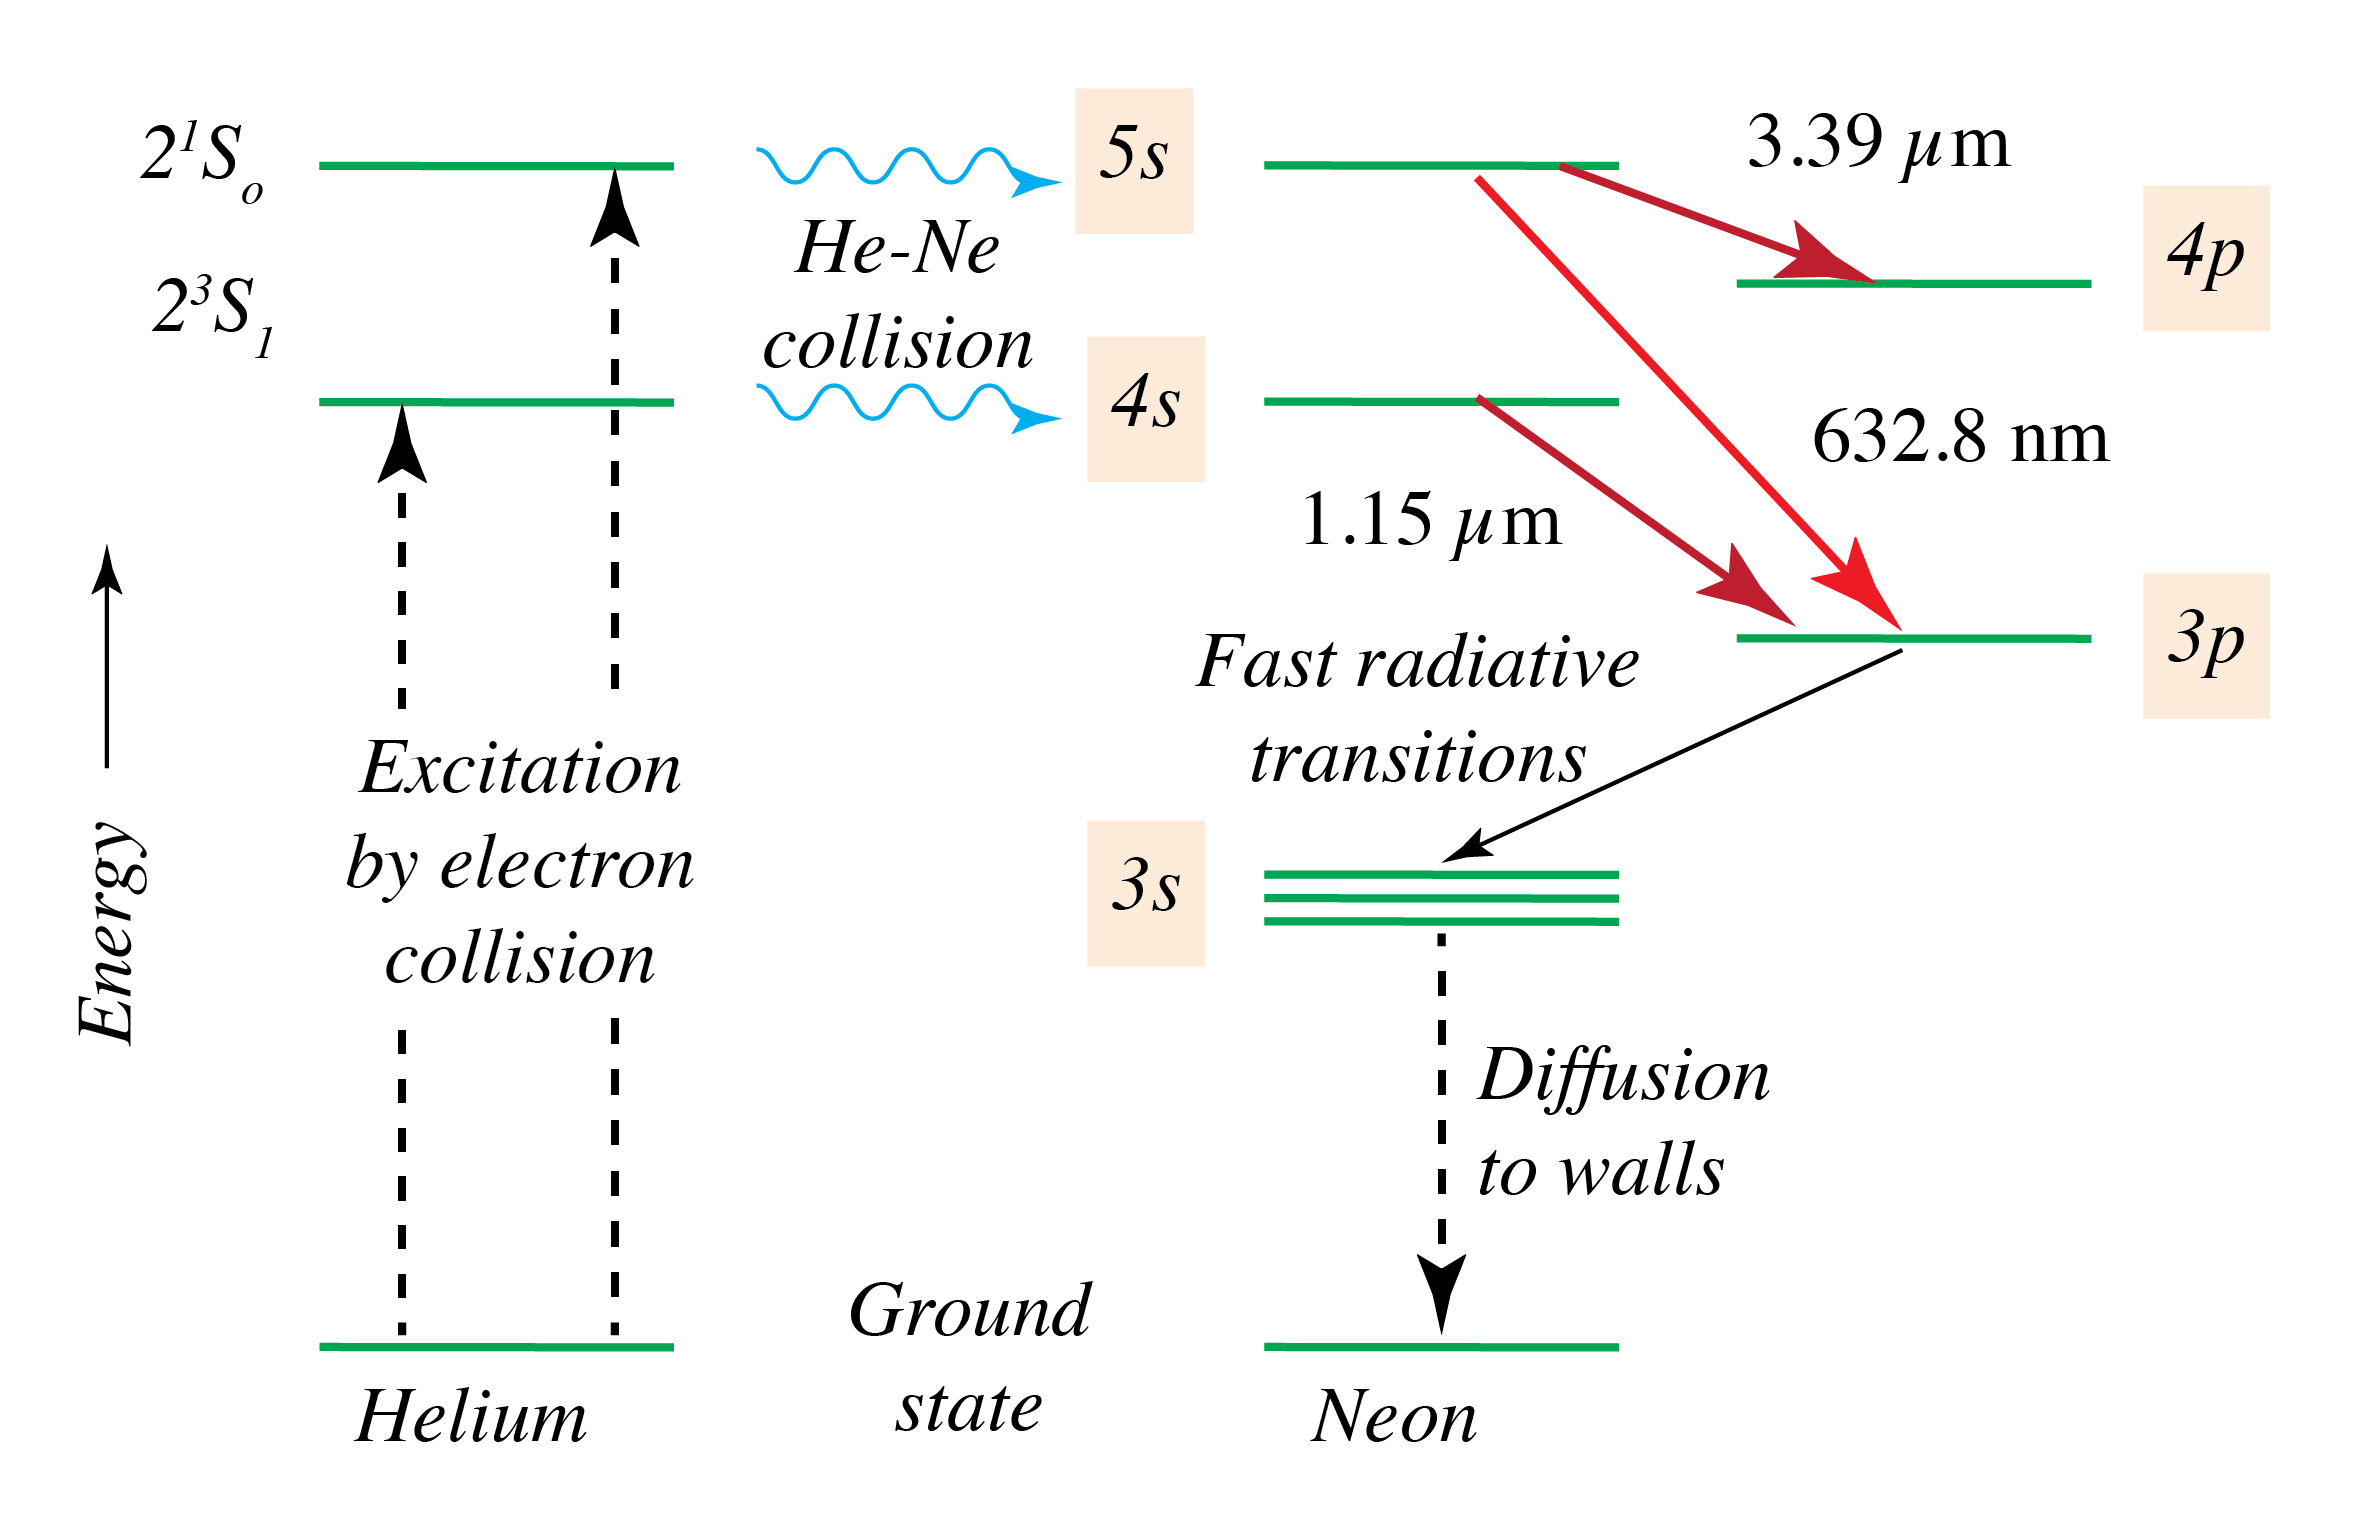
\includegraphics[width=0.6\linewidth]{images/APL1_8_HeNe_Laser_Levels}
				\caption{Energy levels in a He-Ne Laser (\cite{a}).}
				\label{fig:apl18henelaserlevels}
			\end{figure}
			
			\item 氦氖激光器(简称 He-Ne 激光器)由光学谐振腔(输出镜与全反镜)、工作
			物质(密封在玻璃管里的氦气、氖气)、激励系统(激光电源)构成(分为外腔式、
			\textbf{半腔式}和内腔式)。对 He-Ne激光器而言增益介质就是在毛细管内按一定的
			气压充以适当比例的氦氖气体,当氦氖混合气体被电流激励时,
			与某些谱线对应的上下能级的粒子数发生反转,使
			介质具有增益。介质增益与毛细管长度、内径粗细、两种气体的比例、总气压以
			及放电电流等因素有关。\textbf{对谐振腔而言,腔长要满足频率的驻波条件,谐振腔镜
			的曲率半径要满足腔的稳定条件。总之腔的损耗必须小于介质的增益,才能建立
			激光振荡。}
			\begin{figure}[h]
				\centering
				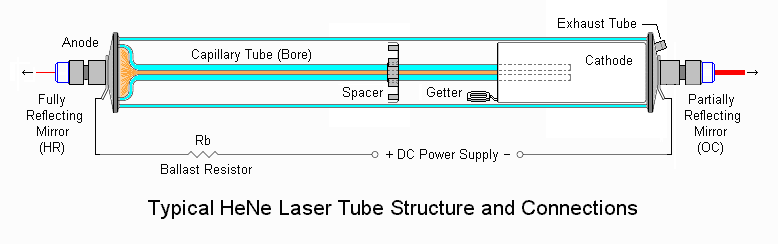
\includegraphics[width=0.7\linewidth]{APL1_8_Typical_HeNe_Laser_Tube_Structure.png}
				\caption{Schematic diagram of a typical 2-3 mW red (633 nm) helium–neon laser tube (\cite{a}).}
				\label{fig:apl18typicalhenelasertubestructure}
			\end{figure}
		\end{itemize}
	\end{itemize}
	
	\item 谐振腔的光场分布
	
	激光由增益介质、光学谐振腔和激励能源组成,\textbf{激光谐振腔有本征频率,每
	一个频率对应一种光场分布,叫做一种模式}。引入\textbf{横模纵模}的概念来描述谐振腔
	内每个本征频率对应的光场分布。谐振腔不同,它的模式就不同。
	
	谐振腔模式可分为两种类型:纵向模式,频率彼此不同;横向模式,频率和光强度模式都不同。纵模描述轴向光场分布状态,横模描述横向分布状态。
	
	谐振腔的\textbf{基本横向模式}是\textbf{高斯光束}(\textbf{详见后})。
	
	谐振腔内的光会在镜子上多次反射,由于干涉效应,谐振腔只能维持某些辐射模式和频率,其他辐射模式和频率则会受到相消干涉的抑制。一般而言,光在谐振腔中每次往返时重现的辐射模式是最稳定的。这些模式被称为谐振腔模式。光在谐振腔中来回反射时,由于工作物质的横截面积和镜面都是有限
	的,当平行光通过它们时,因为衍射作用,使出射光波阵面发生畸变,从而在垂
	直于光的传播方向及横向上,将出现各种不同的场强分布,每一种分布形式叫做
	一种横模。
	
	\begin{figure}[h]
		\centering
		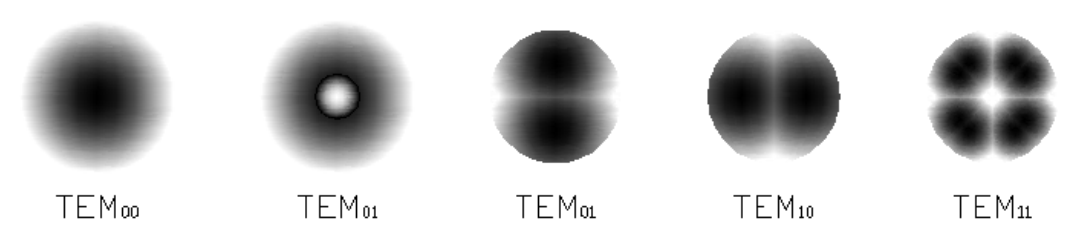
\includegraphics[width=0.7\linewidth]{images/APL1_8_TEM}
		\caption{常见的基本横模光斑图样}
		\label{fig:apl18tem}
	\end{figure}
	
	我们具体来看\textbf{横模}的一些细节:
	\[
	\Delta \nu_{\text{横}} = \frac{c}{2 \mu L} \left\{ \frac{1}{\pi} (\Delta m + \Delta n) \arccos \left[ \sqrt{ \left( 1 - \frac{1}{R_1} \right) \left( 1 - \frac{1}{R_2} \right) } \right] \right\}
	\]
	其中,\( \Delta \nu_{\text{横}} \):横模频率间隔,即不同横模之间的频率差;\( c \):光速(\(3 \times 10^8 \, \text{m/s}\));\( L \):激光谐振腔的长度;\( \mu \):激光介质的折射率(一般取 1 对于真空或气体);\( R_1, R_2 \):谐振腔两端反射镜的曲率半径;\( \Delta m \)、\( \Delta n \):横模的序数差,分别表示在 \(x\) 和 \(y\) 方向上的模序差。
	
	\textbf{考虑这个公式的由来}:
	
	纵模描述光场沿谐振腔轴向的驻波结构。它的频率间隔由谐振腔的长度 \(L\) 和光速 \(c\) 决定:
	\[
	\Delta \nu_{\text{纵}} = \frac{c}{2 \mu L}
	\]
	横模描述光场在谐振腔横截面上的场强分布。谐振腔中的横模结构取决于谐振腔的几何形状、长度以及两端反射镜的曲率半径 \(R_1\) 和 \(R_2\)。
	
	反射镜的曲率决定了光束在腔内的聚焦和散射特性。如果腔内反射镜的曲率半径分别为 \(R_1\) 和 \(R_2\),则光束在传播时会受到这些镜面的约束,影响谐振模的频率分布。
	
	通常采用高斯模式的横模结构表示为 \( \text{TEM}_{mn} \),其中 \(m\) 和 \(n\) 分别为光束在 \(x\) 和 \(y\) 方向上的节点数。不同横模的频率也会有所不同。
	
	谐振腔内的光波必须满足驻波条件,其中 \(q\) 是纵模的整数序数,频率 \( \nu \) 满足:
	\[
	\nu = q \frac{c}{2 L}
	\]
	由于横模的存在,光波的传播路径不再是简单的直线传播,而会受到反射镜曲率的影响。对于两个反射镜曲率分别为 \(R_1\) 和 \(R_2\) 的谐振腔,光波的传播路径可以用下面的表达式修正。
	
	传播路径的弯曲程度反映在模之间的相位延迟上,且这个延迟与 \( \arccos \) 函数相关:
	\[
	\Delta \phi_{\text{横}} = \arccos \left[ \sqrt{ \left( 1 - \frac{1}{R_1} \right) \left( 1 - \frac{1}{R_2} \right) } \right]
	\]
	这个相位延迟与横模频率的间隔有关。由于横模的频率间隔还与模序数 \( \Delta m \) 和 \( \Delta n \) 相关,因此频率间隔可以表示为:
	\[
	\Delta \nu_{\text{横}} = \frac{c}{2 \mu L} \cdot \frac{1}{\pi} (\Delta m + \Delta n) \arccos \left[ \sqrt{ \left( 1 - \frac{1}{R_1} \right) \left( 1 - \frac{1}{R_2} \right) } \right]
	\]
	
	基于上述公式,我们可以考虑“\textbf{通过调节后腔镜改变激光器腔长和模式}”的原理
	
	氦氖激光器的模式结构(包括纵模和横模)受谐振腔的长度和两端反射镜的对准情况影响。\textbf{通过调节后腔镜的齿轮齿条平移台}\textbf{和俯仰偏摆旋钮},可以微调谐振腔的腔长和腔镜的角度,使得激光器内驻波条件发生变化,进而影响激光器的模式(包括横模和纵模)。
	
	齿轮齿条平移台的主要作用是通过\textbf{平移后腔镜}来精确调节谐振腔的长度。  谐振腔长度 \(L\)决定了激光器支持的纵模频率,纵模间隔满足:
	\[
	\Delta \nu_{\text{纵}} = \frac{c}{2L}
	\]
	当移动后腔镜时,谐振腔的长度 \(L\) 发生变化,改变了腔内驻波的条件,从而改变了纵模的数量和频率分布。使用齿轮齿条系统可以微米级地移动后腔镜,改变纵模的频率分布。在腔长变短时,纵模间隔增大;腔长变长时,纵模间隔变小。如果腔长调整得当,谐振腔内只允许一种纵模存在,则输出为\textbf{单纵模激光},具有良好的时间相干性。如果谐振腔的长度不稳定,可能会允许多个纵模同时存在,产生\textbf{多纵模激光}。这时激光器的光谱会变宽,相干性变差。
	
	 俯仰偏摆旋钮用于微调腔镜的角度,确保腔内的激光束与谐振腔的光轴精确对准。即便是极小的偏摆角度变化,也会显著改变谐振腔的模式。 腔镜角度的微调会改变腔内光束的反射路径,从而改变腔内光场的横向分布,使得不同的横模(TEM\(_{mn}\))发生变化。  高阶横模(如 TEM\(_{10}\)、TEM\(_{11}\) 等)更容易激发出来,光斑会呈现复杂的形状(如双峰、四瓣等)。基模(TEM\(_{00}\))更容易占主导地位,光斑呈现高斯分布,发散角最小,光束质量最好。
	 
	 \textbf{使用齿轮齿条平移台改变腔长}:
	 \begin{enumerate}
	 	\item 松开后腔镜的固定螺丝。
	 	\item 通过齿轮齿条平移台微调腔镜位置,缩短或延长谐振腔的长度。
	 	\item 每次微调后,通过观察激光输出的强度和光谱,判断是否出现纵模变化。
	 	\item 若需要单纵模输出,逐步微调腔长,直至只剩下一条谱线。
	 \end{enumerate}
	 
	 \textbf{使用俯仰偏摆旋钮调整腔镜角度}:
	 \begin{enumerate}
	 	\item 打开激光器,并观察光斑形状。
	 	\item 旋转俯仰偏摆旋钮,缓慢调节腔镜的倾角。
	 	\item 调节过程中,观察光斑形状的变化。如果光斑从多峰或非对称分布变为高斯分布(TEM\(_{00}\)),说明光轴对准良好。
	 	\item 若实验需要激发高阶横模,则故意微调腔镜,使光轴稍微偏离对准状态,激发更复杂的横模。
	 \end{enumerate}
	
	\item 高斯光束
	\begin{enumerate}
		\item 基本概念和参数
		
		\textbf{高斯光束}是一种理想的电磁辐射光束,其横向平面内的振幅包络由高斯函数给出;这也意味着高斯强度(辐照度)分布。这种基波(或 TEM 00)横向高斯模式描述了许多激光器的预期输出,因为这种光束发散性较小,并且比任何其他光束都更容易聚焦。当高斯光束被理想透镜重新聚焦时,就会产生新的高斯光束。沿给定波长和偏振的圆形高斯光束的电场和磁场振幅分布由两个参数决定:束腰$w_0$(光束最窄点的宽度度量)和相对于腰部的位置z 。 而我们通常关心的参数有\textbf{光腰位置、光斑半径、远场发散角、瑞利长度}。
		
		\begin{figure}[h]
			\centering
			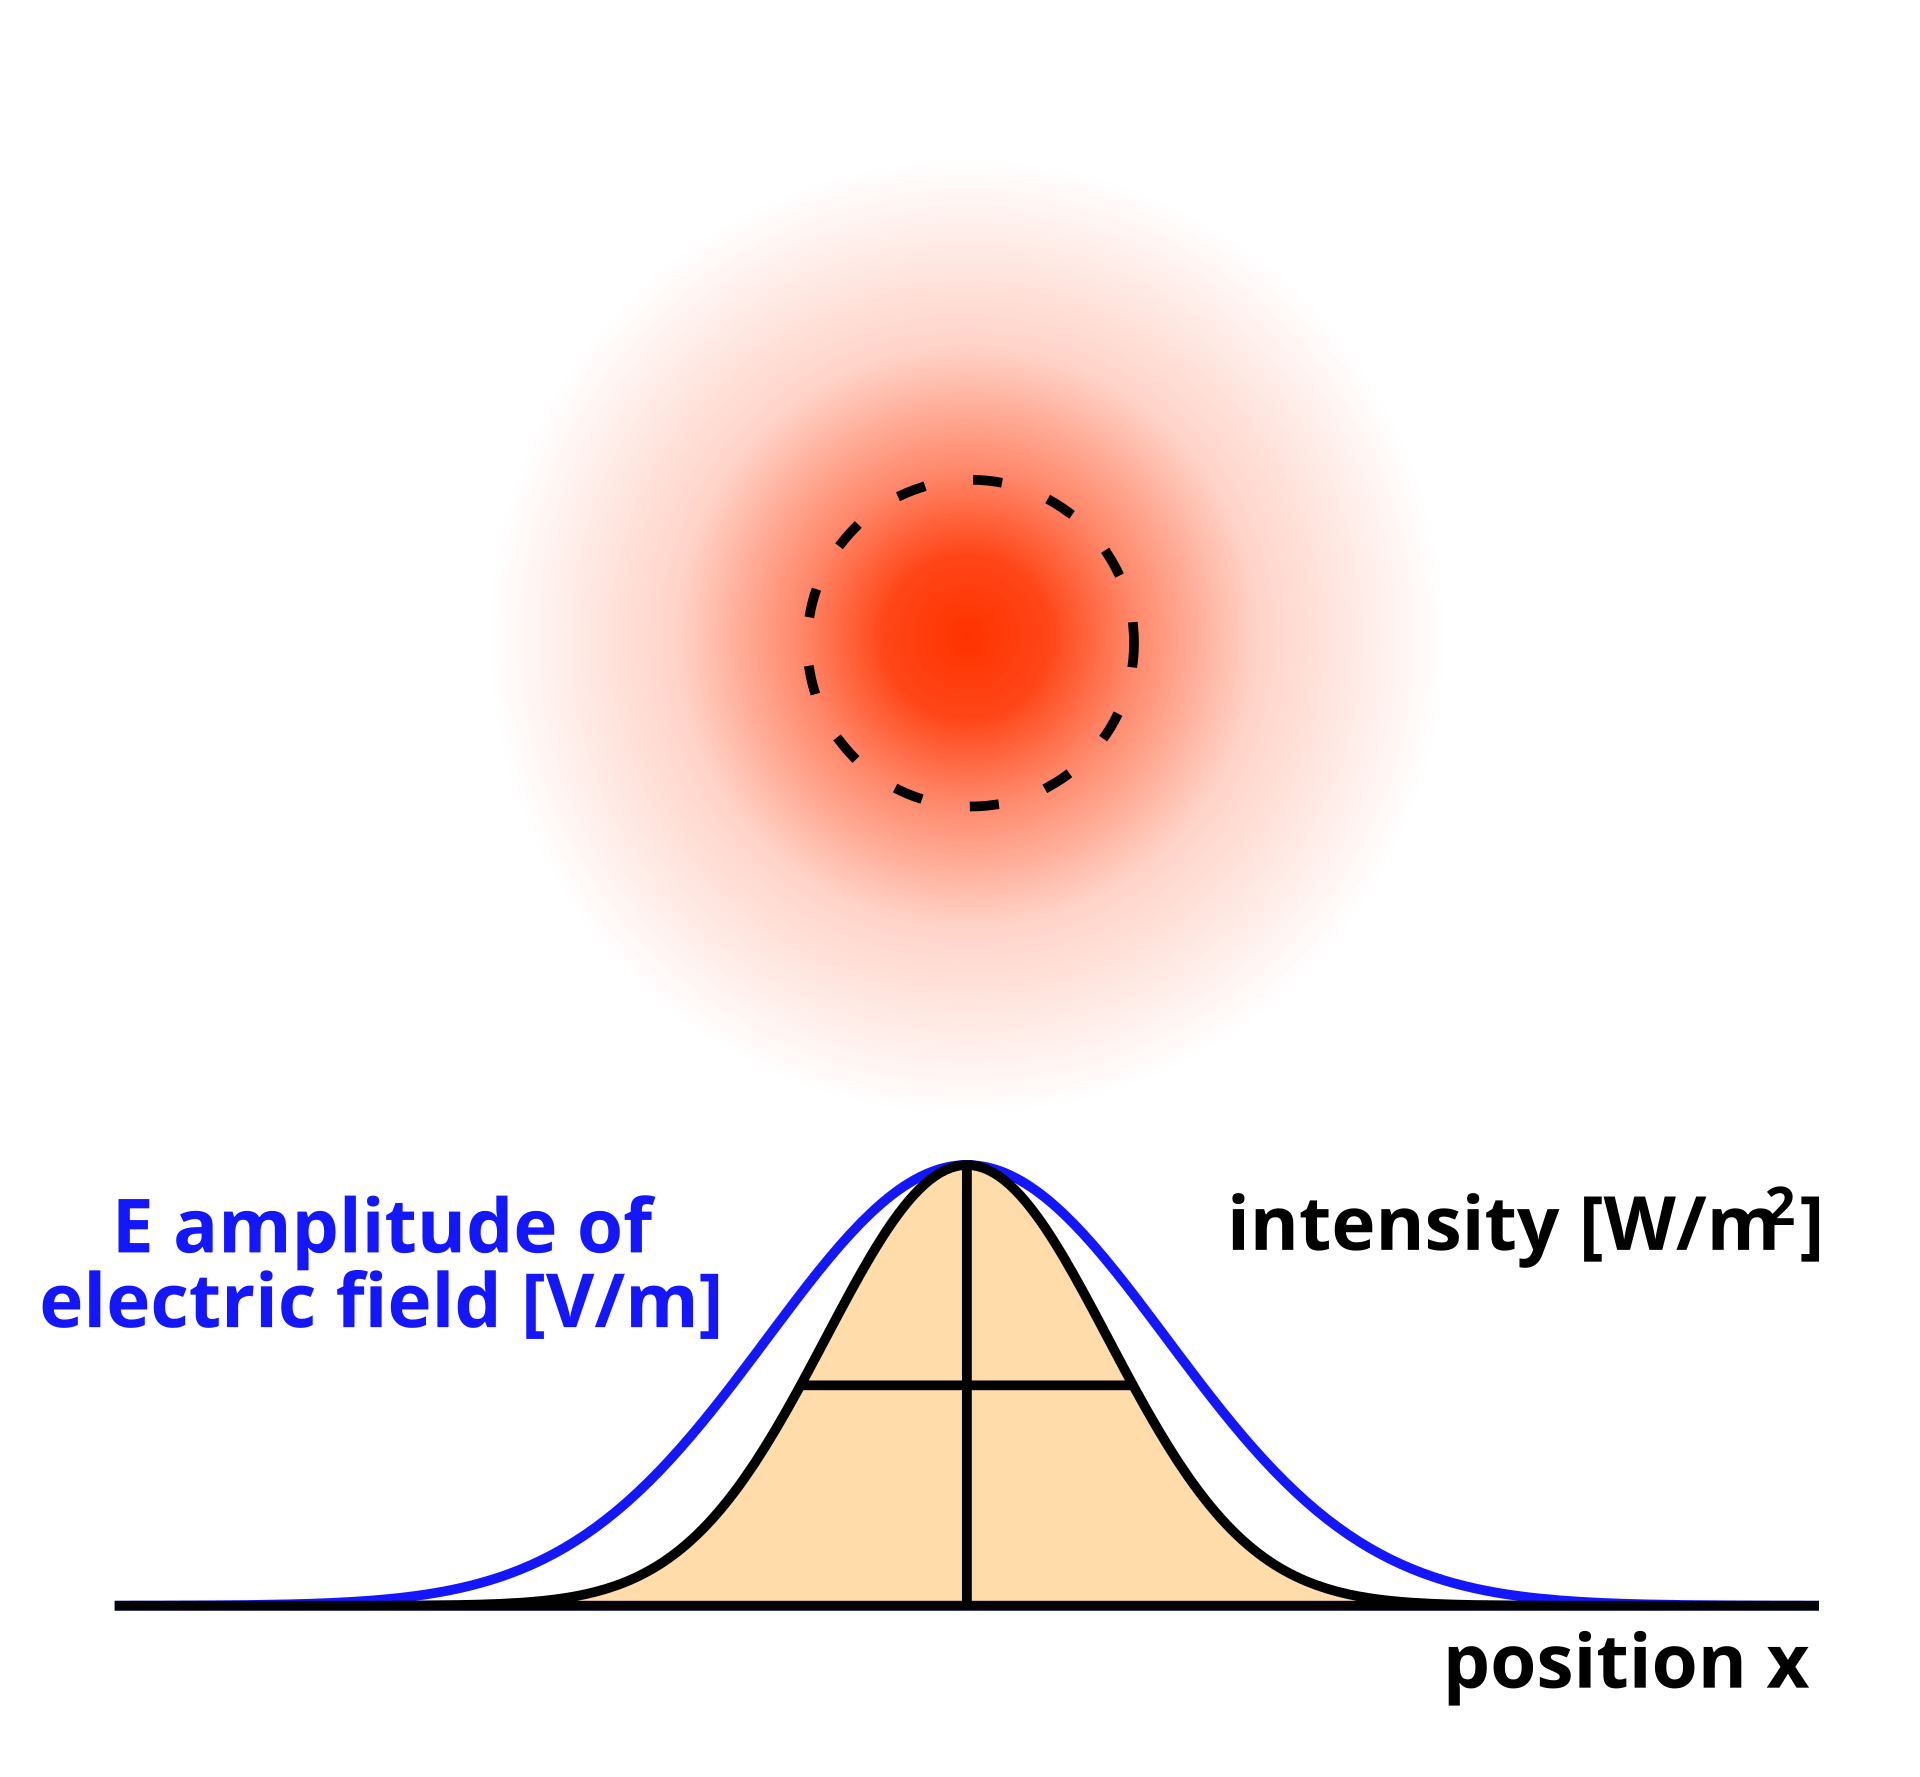
\includegraphics[width=0.35\linewidth]{images/APL1_8_Laser_gaussian_profile}
			\caption{高斯光束}
			\label{fig:apl18lasergaussianprofile}
		\end{figure}
		
		\begin{itemize}
			\item 从根本上讲,高斯光束是\textbf{轴向亥姆霍兹方程在慢变振幅近似下(电磁场的波动方程)的解},以下给出一个\textbf{求解过程}的参考。
			
			首先,考虑电磁波在均匀、各向同性且无源的介质中传播。对于线偏振、单色电磁波,其电场和磁场可以由麦克斯韦方程组描述。在自由空间或均匀介质中,麦克斯韦方程组为:
			
			\[
			\begin{cases}
				\nabla \times \mathbf{E} = -\mu_0 \dfrac{\partial \mathbf{H}}{\partial t}, \\
				\nabla \times \mathbf{H} = \epsilon_0 \dfrac{\partial \mathbf{E}}{\partial t}, \\
				\nabla \cdot \mathbf{E} = 0, \\
				\nabla \cdot \mathbf{H} = 0.
			\end{cases}
			\]
			
			对于无源区域,假设场具有时间简谐性,即\(\mathbf{E}(\mathbf{r}, t) = \mathbf{E}(\mathbf{r}) e^{-i\omega t}\),则麦克斯韦方程组可化简为亥姆霍兹方程:
			
			\[
			\nabla^2 \mathbf{E} + k^2 \mathbf{E} = 0,
			\]
			
			其中,\(k = \omega \sqrt{\mu_0 \epsilon_0}\)为波数。在许多光学问题中,可以采用标量近似,即假设电场只有一个分量,或者各分量彼此独立。这样,亥姆霍兹方程变为标量形式:
			
			\[
			\nabla^2 \psi + k^2 \psi = 0,
			\]
			
			其中,\(\psi\)表示标量场,例如电场的某一分量。
			
			为了求解上述方程,我们\textbf{考虑光束主要沿着\(z\)方向传播,且在横向(\(x\)和\(y\)方向)上的变化相对于\(z\)方向较慢,即近轴近似(paraxial approximation)。}在此近似下,波动方程可以简化为抛物方程。将标量场写为:
			
			\[
			\psi(x, y, z) = u(x, y, z) e^{i k z},
			\]
			
			其中,\(u(x, y, z)\)是包络函数,描述了光束在横向的分布。将\(\psi\)代入标量波动方程,得:
			
			\[
			\nabla^2 [u e^{i k z}] + k^2 u e^{i k z} = 0.
			\]
			
			计算拉普拉斯算符:
			
			\[
			\nabla^2 [u e^{i k z}] = e^{i k z} \left( \nabla^2 u + 2 i k \dfrac{\partial u}{\partial z} - k^2 u \right).
			\]
			
			代入后得到:
			
			\[
			e^{i k z} \left( \nabla^2 u + 2 i k \dfrac{\partial u}{\partial z} \right) = 0.
			\]
			
			\begin{ubox}{}
				因此,\textbf{得到近轴标量波动方程}:
				
				\[
				\nabla_\perp^2 u + 2 i k \dfrac{\partial u}{\partial z} = 0,
				\]
				
				其中,\(\nabla_\perp^2 = \dfrac{\partial^2}{\partial x^2} + \dfrac{\partial^2}{\partial y^2}\)是横向拉普拉斯算符。
			\end{ubox}
			
			为了解决这个方程,我们寻找满足上述抛物方程的函数形式。考虑圆对称情况,即\textbf{光束在横向具有圆对称性},\(u\)仅依赖于径向坐标\(r = \sqrt{x^2 + y^2}\)。因此,方程变为:
			
			\[
			\left( \dfrac{1}{r} \dfrac{\partial}{\partial r} \left( r \dfrac{\partial u}{\partial r} \right) \right) + 2 i k \dfrac{\partial u}{\partial z} = 0.
			\]
			
			假设解的形式为:
			
			\[
			u(r, z) = A(z) e^{- \dfrac{r^2}{w^2(z)}},
			\]
			
			其中,\(A(z)\)是幅度,\textbf{\(w(z)\)是光束半径},都是关于\(z\)的函数。首先计算\(\dfrac{\partial u}{\partial z}\):
			
			\[
			\dfrac{\partial u}{\partial z} = \left( \dfrac{d A}{d z} - A \dfrac{2 r^2}{w^3} \dfrac{d w}{d z} \right) e^{- \dfrac{r^2}{w^2}}.
			\]
			
			其次,计算径向拉普拉斯项:
			
			\[
			\dfrac{\partial u}{\partial r} = - \dfrac{2 r A}{w^2} e^{- \dfrac{r^2}{w^2}},
			\]
			
			\[
			\dfrac{\partial}{\partial r} \left( r \dfrac{\partial u}{\partial r} \right) = - \dfrac{2 A}{w^2} e^{- \dfrac{r^2}{w^2}} \left( 2 \dfrac{r^2}{w^2} - 1 \right).
			\]
			
			因此,径向拉普拉斯算符为:
			
			\[
			\left( \dfrac{1}{r} \dfrac{\partial}{\partial r} \left( r \dfrac{\partial u}{\partial r} \right) \right) = - \dfrac{2 A}{w^2} e^{- \dfrac{r^2}{w^2}} \left( 2 \dfrac{r^2}{w^2} - 1 \right).
			\]
			
			将以上结果代入近轴方程:
			
			\[
			- \dfrac{2 A}{w^2} \left( 2 \dfrac{r^2}{w^2} - 1 \right) + 2 i k \left( \dfrac{d A}{d z} - A \dfrac{2 r^2}{w^3} \dfrac{d w}{d z} \right) = 0.
			\]
			
			将\(e^{- \dfrac{r^2}{w^2}}\)约去,并整理得到:
			
			\[
			- \dfrac{2 A}{w^2} \left( 2 \dfrac{r^2}{w^2} - 1 \right) + 2 i k \left( \dfrac{d A}{d z} - A \dfrac{2 r^2}{w^3} \dfrac{d w}{d z} \right) = 0.
			\]
			
			为了使方程在\(r\)的各次幂上成立,我们将同次幂的项收集。常数项(与\(r^0\)有关):
			
			\[
			\dfrac{2 A}{w^2} + 2 i k \dfrac{d A}{d z} = 0.
			\]
			
			\(r^2\)项:
			
			\[
			- \dfrac{4 A r^2}{w^4} - 4 i k A \dfrac{r^2}{w^3} \dfrac{d w}{d z} = 0.
			\]
			
			将\(r^2\)项整理为:
			
			\[
			\left( - \dfrac{4 A}{w^4} - \dfrac{4 i k A}{w^3} \dfrac{d w}{d z} \right) r^2 = 0.
			\]
			
			要使上述等式对任意\(r\)成立,必须令各系数为零。从\(r^2\)项微分方程:
			
			\[
			- \dfrac{4 A}{w^4} - \dfrac{4 i k A}{w^3} \dfrac{d w}{d z} = 0.
			\]
			
			两边除以\(-4 A\),得到:
			
			\[
			\dfrac{1}{w^4} + i k \dfrac{1}{w^3} \dfrac{d w}{d z} = 0.
			\]
			
			乘以\(w^4\):
			
			\[
			1 + i k w \dfrac{d w}{d z} = 0.
			\]
			
			整理得到:
			
			\[
			i k w \dfrac{d w}{d z} = -1.
			\]
			
			两边乘以\(i\):
			
			\[
			- k w \dfrac{d w}{d z} = - i \implies k w \dfrac{d w}{d z} = i.
			\]
			
			因此,
			
			\[
			\dfrac{d w^2}{d z} = \dfrac{2 i}{k}.
			\]
			
			因为\(\dfrac{d w^2}{d z} = 2 w \dfrac{d w}{d z}\),所以:
			
			\[
			\dfrac{d w^2}{d z} = \dfrac{2 i}{k}.
			\]
			
			积分得到:
			
			\[
			w^2(z) = w_0^2 + \dfrac{2 i}{k} z,
			\]
			
			其中,\textbf{\(w_0\)是\(z = 0\)处的光束半径}。为了方便,我们将其写为:
			
			\[
			w^2(z) = w_0^2 \left( 1 + \dfrac{2 i z}{k w_0^2} \right).
			\]
			
			定义\textbf{瑞利长度}:
			
			\[
			z_R = \dfrac{k w_0^2}{2} = \dfrac{\pi w_0^2}{\lambda},
			\]
			
			因此,
			
			\[
			w^2(z) = w_0^2 \left( 1 + i \dfrac{z}{z_R} \right).
			\]
			
			但由于\(w^2(z)\)必须是实数,因此需要考虑复数参数的物理意义。实际上,我们引入曲率半径\(R(z)\)和桂馥相位\(\zeta(z)\),并定义复参数\(q(z)\):
			
			\[
			\dfrac{1}{q(z)} = \dfrac{1}{R(z)} - i \dfrac{\lambda}{\pi w^2(z)}.
			\]
			
			回到常数项微分方程:
			
			\[
			\dfrac{2 A}{w^2} + 2 i k \dfrac{d A}{d z} = 0.
			\]
			
			整理为:
			
			\[
			\dfrac{1}{A} \dfrac{d A}{d z} = - \dfrac{i}{k w^2(z)}.
			\]
			
			我们已经知道\(w^2(z)\),可以求解\(A(z)\)。积分得到:
			
			\[
			\ln A = - \int \dfrac{i}{k w^2(z)} d z + C \implies A(z) = A_0 e^{- \int \dfrac{i}{k w^2(z)} d z}.
			\]
			
			由于积分可能比较复杂,而在光束传播过程中,幅度的变化通常与光束半径的倒数成正比,即:
			
			\[
			A(z) \propto \dfrac{1}{w(z)}.
			\]
			
			因此,可以得出:
			
			\[
			A(z) = \dfrac{A_0}{w(z)}.
			\]
			
			综合以上结果,高斯光束的解为:
			
			\[
			\psi(r, z) = A_0 \dfrac{1}{w(z)} \exp \left( - \dfrac{r^2}{w^2(z)} \right) e^{i k z}.
			\]
			
			为了更精确地描述光束的相位变化,引入曲率半径\(R(z)\)和桂馥相位\(\zeta(z)\)。
			
			\textbf{曲率半径}定义为:
			
			\[
			R(z) = z \left( 1 + \left( \dfrac{z_R}{z} \right)^2 \right).
			\]
			
			\textbf{桂馥相位}定义为:
			
			\[
			\zeta(z) = \arctan \left( \dfrac{z}{z_R} \right).
			\]
			
			\begin{ubox}{}
				因此,\textbf{完整的高斯光束表达式}为:
				
				$$
				\psi(r, z) = A_0 \dfrac{w_0}{w(z)} \exp \left( - \dfrac{r^2}{w^2(z)} \right) \exp \left( - i k \dfrac{r^2}{2 R(z)} \right) \exp \left[ i \left( k z - \zeta(z) \right) \right],
				$$
				
				其中:
				\begin{itemize}
					\item $z_R = \frac{\pi w_0^2}{\lambda}$,为瑞利尺寸(共焦参数);
					\item \(w(z) = w_0 \sqrt{1 + \left( \dfrac{z}{z_R} \right)^2 }\),为高斯光束的束宽;
					\item \(R(z) = z \left( 1 + \left( \dfrac{z_R}{z} \right)^2 \right)\),为高斯光束的等相面曲率半径;
					\item \(\zeta(z) = \arctan \left( \dfrac{z}{z_R} \right)\),为高斯光束的相位因子。
				\end{itemize}
			\end{ubox}
			
			\item 接下来我们基于上述公式,对各参数进行细致的讨论:
			\begin{equation*}
				\mathbf{E}(r,z) = E_0 \, \hat{\mathbf{x}} \, \frac{w_0}{w(z)}\exp \left( \frac{-r^2}{w(z)^2} \right)\exp \left(\! -i \left(kz +k \frac{r^2}{2R(z)} - \psi(z) \right)\!\right)
			\end{equation*}
			
			\begin{itemize}
				\item $r$ 是距离光束中心轴的径向距离,
				\item $z$ 是距离光束焦点(或称“腰部”)的轴向距离,
				\item $i$ 是虚数单位,
				\item $k = \frac{2\pi n}{\lambda}$ 是自由空间波长 $\lambda$ 对应的波数(以弧度每米为单位),其中 $n$ 是光束传播介质的折射率,
				\item $E_0 = E(0, 0)$ 是在原点(即 $r = 0$,$z = 0$)处的电场幅度,
				\item $w(z)$ 是在平面 $z$ 处,场的幅度衰减到其轴向值的 $1/e$ 位置的半径(即强度衰减到其轴向值的 $1/e^2$ 位置的半径),
				\item $w_0 = w(0)$ 是光束的腰部半径,
				\item $R(z)$ 是在 $z$ 处光束波前的曲率半径,
				\item $\psi(z) = \arctan\left(\frac{z}{z_R}\right)$ 是 $z$ 处的 Gouy 相位,是相对于光的相速的一个附加相位项。
			\end{itemize}
			
			物理电场可以通过从上面给出的相量场幅度取其实部,并乘以一个时间因子来获得:
			\[
			\mathbf{E}_\text{phys}(r,z,t) = \operatorname{Re} \left( \mathbf{E}(r,z) \cdot e^{i\omega t} \right),
			\]
			其中 $\omega$ 是光的角频率,$t$ 是时间。
			
			由于此解依赖于近轴近似,因此对于强烈发散的光束不够准确。但在大多数实际情况下,上述形式是有效的,即当 $w_0 \gg \frac{\lambda}{n}$。
			
			对应的\textbf{强度}(或辐照度)分布由下式给出:
			\[
			I(r, z) = \frac{|\mathbf{E}(r, z)|^2}{2 \eta} = I_0 \left( \frac{w_0}{w(z)} \right)^2 \exp \left( \frac{-2r^2}{w(z)^2} \right),
			\]
			其中常数 $\eta$ 是光束传播介质的波阻抗。对于自由空间,$\eta = \eta_0 \approx 377 \, \Omega$。$I_0 = \frac{|E_0|^2}{2 \eta}$ 是光束在腰部中心处的强度。
			
			如果 $P_0$ 是光束的总功率,那么有:
			\[
			I_0 = \frac{2 P_0}{\pi w_0^2}.
			\]
			
			在上述参数中,我们又特别关注所谓的“梁参数(或者束腰参数,Beam Parameters)”。给定波长 $\lambda$ 的高斯光束形状由一个参数——\textbf{光束腰半径} $w_0$ 唯一决定。光束腰是光束在焦点处(即 $z = 0$)的尺寸,此处的光束宽度 $w(z)$ 达到最小值,而轴线上(即 $r = 0$)的强度达到最大值。从这一参数可以确定描述光束几何结构的其他参数,包括瑞利区间 $z_R$ 和渐近角发散 $\theta$,如下所述。
			
			\begin{figure}[h]
				\centering
				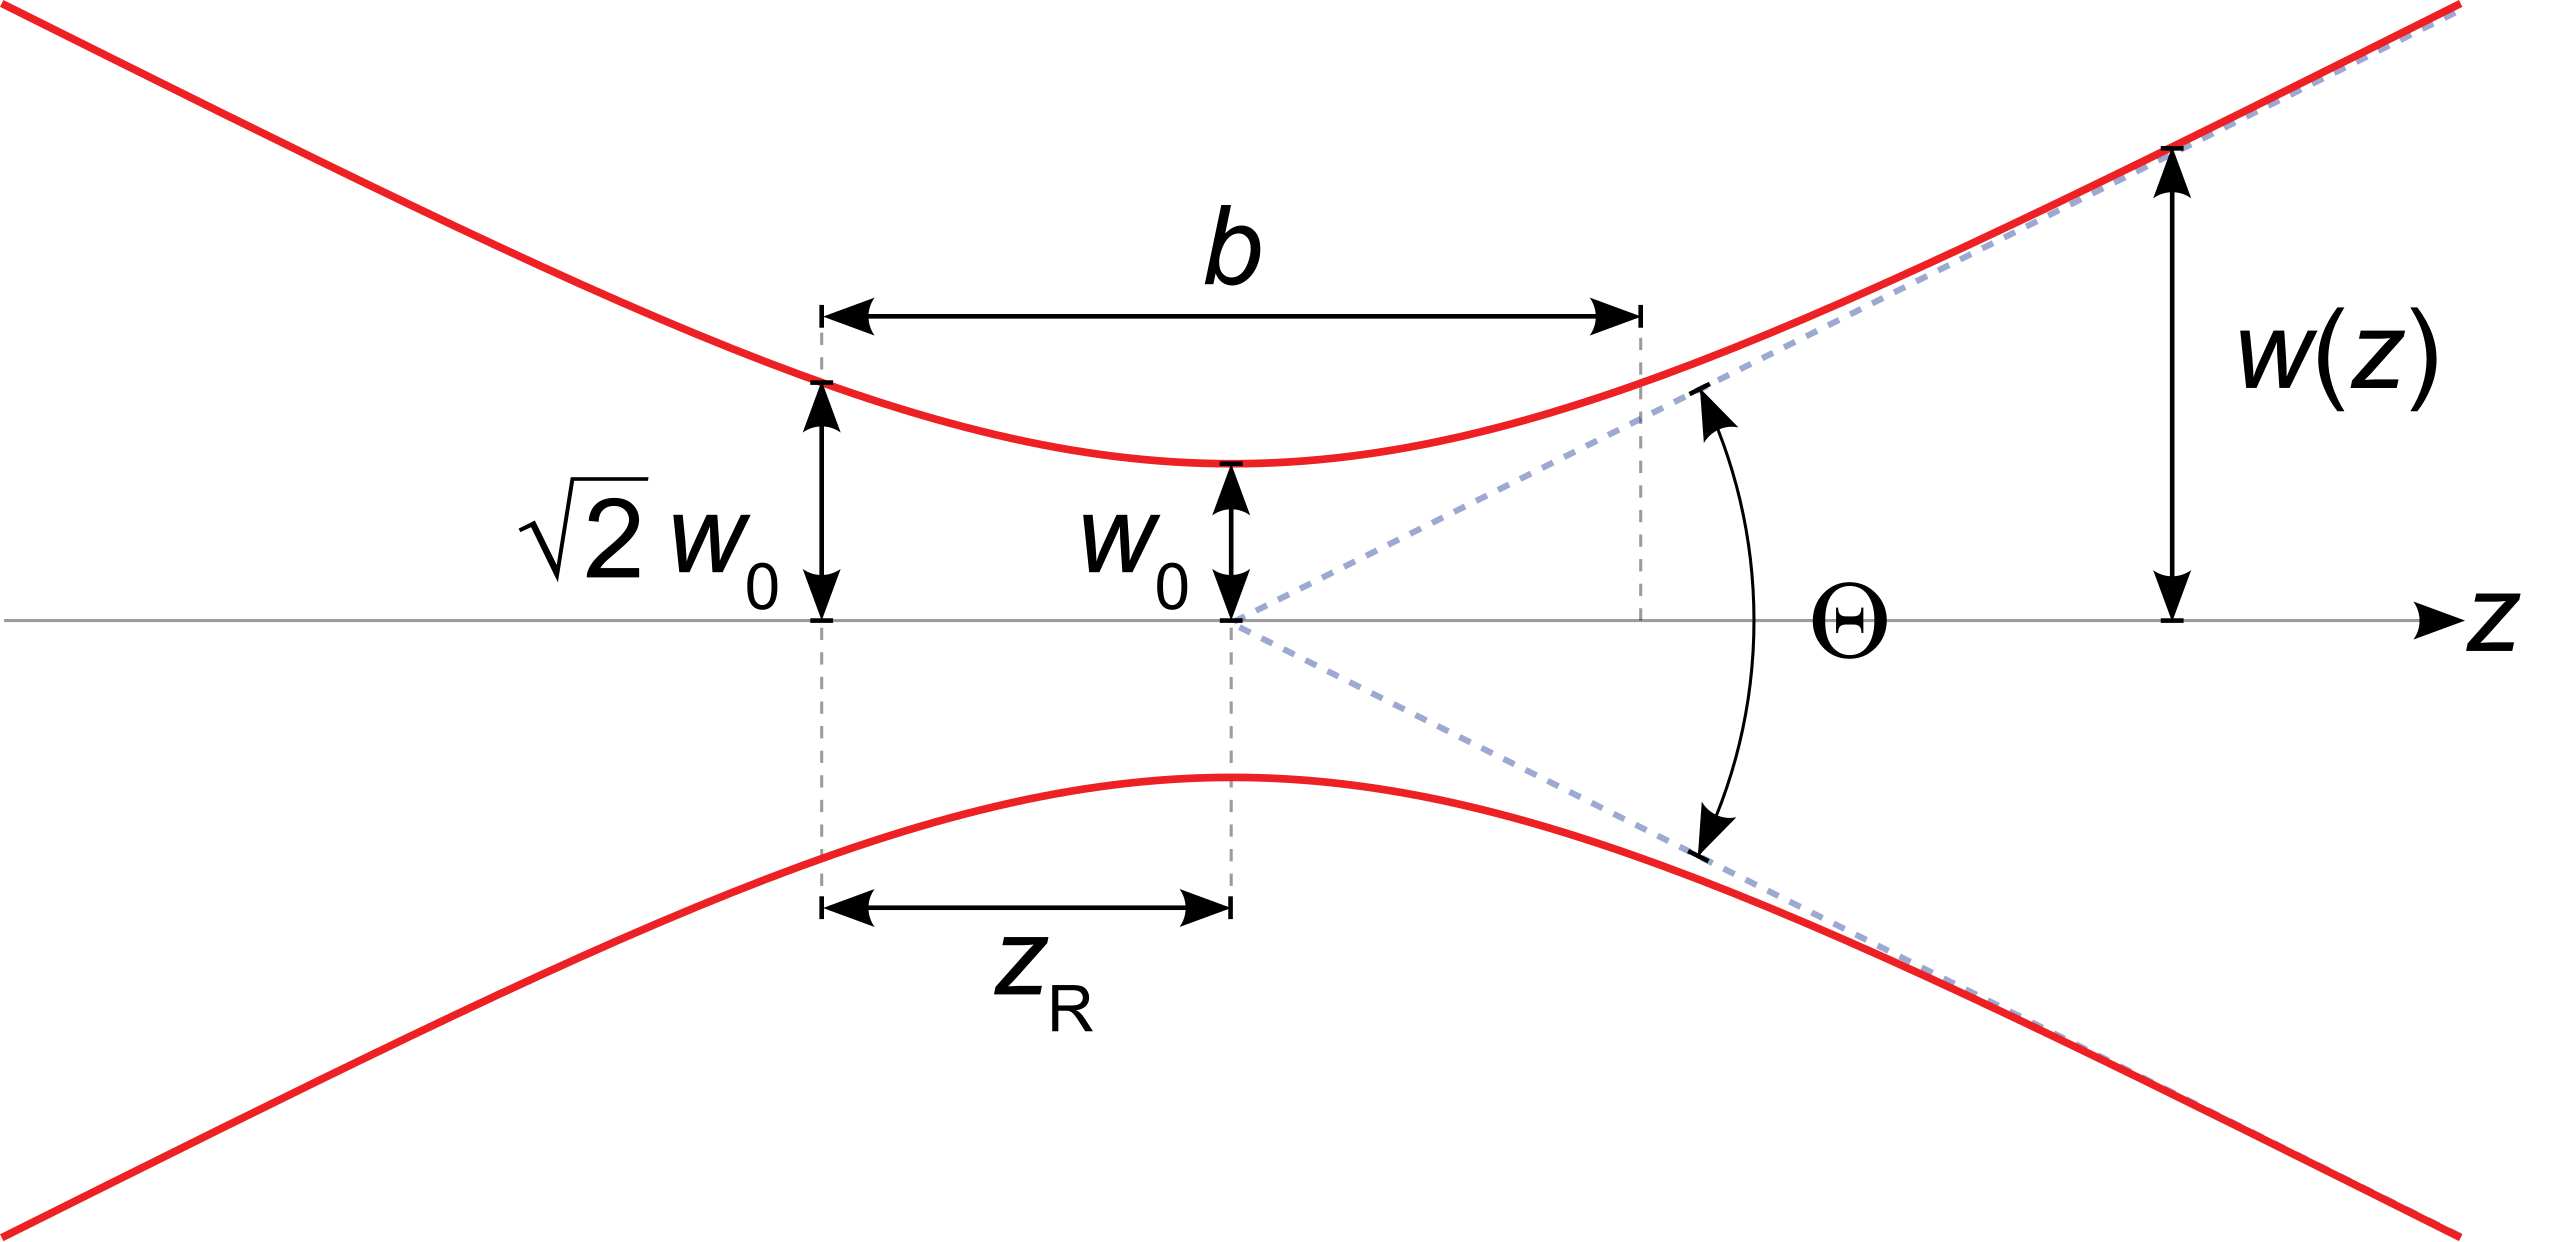
\includegraphics[width=0.7\linewidth]{images/APL1_8_GaussianBeamWaist}
				\caption{高斯光束宽度$w(z)$随沿光束传播方向距离$z$的变化呈现双曲线形状。$w_0$:光束腰半径;$b$:焦深;$z_R$:瑞利区间;$\Theta$:光束的总角发散。(\cite{a})}
				\label{fig:apl18gaussianbeamwaist}
			\end{figure}
			
			瑞利距离或瑞利区间 $z_R$ 由高斯光束的腰部半径决定:
			\[
			z_R = \frac{\pi w_0^2 n}{\lambda}.
			\]
			其中,$\lambda$ 是光的波长,$n$ 是介质的折射率。在距离腰部等于瑞利区间 $z_R$ 的位置,光束的宽度 $w$ 是焦点处($w = w_0$)的 $\sqrt{2}$ 倍。这也意味着,在该处轴线上($r = 0$)的强度是峰值强度($z = 0$ 处)的二分之一。该点也是波前曲率($1/R$)达到最大值的地方。
			
			两点 $z = \pm z_R$ 之间的距离被称为光束的\textbf{共焦参数}或\textbf{焦深}。
			
			尽管高斯函数的尾部实际上永远不会达到零,但在以下讨论中,光束的“边缘”被认为是半径 $r = w(z)$ 处的位置,即强度降至其轴线上最大值的 $1/e^2$ 处。当 $z \gg z_R$ 时,$w(z)$ 线性增加。这意味着在远离光束腰部的地方,光束的“边缘”(以上述定义)呈锥形。锥形边缘与光束轴线(即 $r = 0$)之间的夹角定义了光束的\textbf{发散角}:
			
			\[
			\theta = \lim_{z \to \infty} \arctan\left(\frac{w(z)}{z}\right).
			\]
			
			在近轴近似的情况下,发散角 $\theta$(以弧度为单位)可以近似为:
			\[
			\theta = \frac{\lambda}{\pi n w_0},
			\]
			其中,$n$ 是光束传播介质的折射率,$\lambda$ 是自由空间波长。发散光束的总角扩展(即上述锥形的顶角)则为:
			\[
			\Theta = 2 \theta\,.
			\]
			
			该锥形内包含了 86\% 的高斯光束总功率。
			
			由于发散角与光斑尺寸成反比,因此对于给定的波长 $\lambda$,聚焦至较小光斑的高斯光束在远离焦点时会迅速发散。相反,为了\textbf{最小化}远场发散(并在较大距离处增加峰值强度),光束腰部($w_0$)必须具有较大的横截面(即发射处的直径也需较大,因为 $w(z) \geq w_0$)。这种光束宽度与发散之间的关系是\textbf{衍射}和描述\textbf{夫琅禾费衍射}的\textbf{傅里叶变换}的基本特性。任何指定的幅度分布的光束也遵循这种反比关系,但对于高斯模式而言,焦点处光束尺寸与远场发散角的乘积比其他任何情况都小。
			
			由于高斯光束模型使用了近轴近似,当波前相对于光束轴倾斜超过约 30° 时,该模型不再适用。这意味着根据发散角的表达式,当腰部半径小于约 $2\lambda / \pi$ 时,高斯光束模型将失效。
			
			\textbf{激光光束质量}通过\textbf{光束参数乘积}(BPP)来量化。对于高斯光束,BPP 是光束的发散角和腰部半径 $w_0$ 的乘积。实际光束的 BPP 通过测量其最小直径和远场发散角并取其乘积得到。实际光束的 BPP 与相同波长下理想高斯光束的 BPP 的比值称为 $M^2$ 值(``M 平方'')。对于理想的高斯光束,$M^2 = 1$。所有实际激光光束的 $M^2$ 值均大于 1,但高质量光束的 $M^2$ 值可以非常接近 1。
			
			\textbf{高斯光束的数值孔径}定义为 $NA = n \sin \theta$,其中 $n$ 是光束传播介质的折射率。这意味着瑞利区间与数值孔径的关系为:
			\[
			z_R = \frac{n w_0}{\mathrm{NA}}.
			\]
			
			\textbf{Gouy 相位}是光束在焦点区域附近逐渐获得的相位偏移。在位置 $z$ 处,基模高斯光束的 Gouy 相位为:
			\[
			\psi(z) = \arctan \left( \frac{z}{z_\mathrm{R}} \right).
			\]
			
			Gouy 相位导致光束在腰部附近(即 $z \approx 0$)的\textbf{表观波长}增加。因此,在该区域内的相速度形式上超出了光速。这种看似悖论的行为应被理解为一种\textbf{近场现象}:在绝大多数情况下,相速度与光速(在平面波中精确适用的速度)之间的偏差非常小,除非光束具有较大的\textbf{数值孔径}。在这种情况下,波前曲率在单个波长的距离内会发生显著变化。无论在何种情况下,\textbf{波动方程}在每个位置都得到满足。
			
			Gouy 相位的符号取决于电场相量的符号约定。若采用 $e^{i\omega t}$ 形式,则 Gouy 相位从 $-\pi/2$ 变化为 $+\pi/2$;若采用 $e^{-i\omega t}$ 形式,则相位从 $+\pi/2$ 变化为 $-\pi/2$。
			
			对于基模高斯光束,从腰部一侧的远场到另一侧的远场,Gouy 相位引入了相对于光速的 $\pi$ 弧度(即一个相位反转)的净相位差。这种相位变化在大多数实验中不可观察。然而,在理论上它非常重要,并且对于\textbf{高阶高斯模式}的光束来说,这种相位变化的范围更大。
			
			\item \textbf{综上所述,高斯光束为截面光强呈高斯分布的光束。高斯光束的光束半径随
			坐标 z 呈双曲函数变化;在光腰位置的光束半径达到最小;在远场情况,高斯光
			束有近衍射极限的固定发散角。在旁轴情况下,光束的等相面为球面。在瑞利长
			度范围内,高斯光束可以近似为平行光和平面波。}
			
			\item \textbf{高斯光束参数拟合方法}
			
			根据 \texttt{ISO11146} 文件(实验讲义中提到的)要求,在测量光束传播参数时,沿光束传播轴,至少需要在十个不同位置上测量光斑直径,然后用双曲线拟合的方法求出光束参数。
			
			双曲线拟合方程为:
			\[
			w^2(z) = A + Bz + Cz^2 \quad (w(z) \text{为} z \text{位置的束宽})
			\]
			这些测量位置\textbf{半数应位于束腰两侧一倍瑞利长度之内,其它测量位置在超过一倍瑞利长度之外}。
			
			拟合求解出 $A, B, C$ 以后,可通过\cref{tab:eq}公式计算得到相应的\textbf{光束参数}:
			
			\begin{table}[h!]
				\centering
				\caption{光束参数的计算公式}
				\label{tab:eq}
				\begin{tabular}{|c|c|}
					\hline
					\textbf{光腰位置} & $z_0 = -\frac{B}{2C}$ \\
					\hline
					\textbf{光腰半径} & $\omega_0 = \sqrt{A - \frac{B^2}{4C}}$ \\
					\hline
					\textbf{远场发散角} & $\theta = \sqrt{C}$ \\
					\hline
					\textbf{瑞利长度} & $Z_0 = \frac{1}{2C} \sqrt{4AC - B^2}$ \\
					\hline
				\end{tabular}
			\end{table}
		\end{itemize}
		
		
		\item 高斯光束的“Complex Beam Parameter”(q参数描述)
		
		高斯光束的光斑尺寸和曲率可以通过复光束参数 $q(z)$ 进行编码,并作为 $z$ 的函数给出:
		\[
		q(z) = z + i z_\mathrm{R}.
		\]
		
		复光束参数的倒数包含了波前曲率和轴线上相对强度的实部与虚部:
		\[
		\frac{1}{q(z)} = \frac{1}{R(z)} - i \frac{\lambda}{n \pi w^2(z)}.
		\]
		
		复光束参数简化了高斯光束传播的数学分析,特别是在使用\textbf{光线传递矩阵}分析\textbf{光学谐振腔}时。
		
		使用这种形式,上述电场(或磁场)方程可以大大简化。如果我们用 $u$ 表示椭圆高斯光束的相对场强(椭圆轴沿 $x$ 和 $y$ 方向),则它可以在 $x$ 和 $y$ 方向上分离表示为:
		\[
		u(x, y, z) = u_x(x, z) \, u_y(y, z),
		\]
		其中
		\[
		\begin{aligned}
			u_x(x, z) &= \frac{1}{\sqrt{q_x(z)}} \exp\left(-i k \frac{x^2}{2 q_x(z)}\right), \\
			u_y(y, z) &= \frac{1}{\sqrt{q_y(z)}} \exp\left(-i k \frac{y^2}{2 q_y(z)}\right),
		\end{aligned}
		\]
		其中 $q_x(z)$ 和 $q_y(z)$ 是 $x$ 和 $y$ 方向上的复光束参数。
		
		对于具有\textbf{圆对称}的光束轮廓的常见情况,有 $q_x(z) = q_y(z) = q(z)$,并且 $x^2 + y^2 = r^2$,因此得到:
		\[
		u(r, z) = \frac{1}{q(z)} \exp\left( -i k \frac{r^2}{2 q(z)} \right).
		\]
		
		\item 高斯光束的传播
		
		矩阵可以用于计算高斯光束通过使用相同的传输矩阵描述的光学元件传播时的演化。对于具有波长 $\lambda_0$、曲率半径 $R$(发散时为正,收敛时为负)、光斑尺寸 $w$ 以及折射率 $n$ 的高斯光束,可以定义\textbf{复光束参数} $q$ 为:
		\[
		\frac{1}{q} = \frac{1}{R} - \frac{i \lambda_0}{\pi n w^2}.
		\]
		
		($R$、$w$ 和 $q$ 都是位置的函数。)如果光束轴沿 $z$ 方向,光束腰部位于 $z_0$,瑞利区间为 $z_R$,则复光束参数可以等价表示为:
		\[
		q = (z - z_0) + i z_R.
		\]
		
		该光束可以通过具有给定光线传递矩阵的光学系统传播,使用如下方程:
		\[
		\begin{bmatrix}
			q_2 \\
			1
		\end{bmatrix}
		= k \begin{bmatrix}
			A & B \\
			C & D
		\end{bmatrix}
		\begin{bmatrix}
			q_1 \\
			1
		\end{bmatrix},
		\]
		其中 $k$ 是归一化常数,用于使光线向量的第二个分量保持为 $1$。通过\textbf{矩阵乘法},上述方程展开为:
		\[
		\begin{aligned}
			q_2 &= k (A q_1 + B), \\
			1   &= k (C q_1 + D).
		\end{aligned}
		\]
		
		将第一式除以第二式,可以消去归一化常数:
		\[
		q_2 = \frac{A q_1 + B}{C q_1 + D}.
		\]
		
		通常可以将该方程以倒数形式表示为:
		\[
		\frac{1}{q_2} = \frac{C + D/q_1}{A + B/q_1}.
		\]
		
		\textbf{示例:自由空间传播}
		
		考虑光束在自由空间中传播距离 $d$,其光线传递矩阵为:
		\[
		\begin{bmatrix}
			A & B \\
			C & D
		\end{bmatrix}
		= \begin{bmatrix}
			1 & d \\
			0 & 1
		\end{bmatrix}.
		\]
		因此,
		\[
		q_2 = \frac{A q_1 + B}{C q_1 + D} = \frac{q_1 + d}{1} = q_1 + d,
		\]
		这与普通高斯光束传播的表达式一致,即 $q = (z - z_0) + i z_R$。随着光束的传播,其曲率半径和光束腰部都会发生变化。
		
		\textbf{示例:薄透镜}
		
		考虑光束通过焦距为 $f$ 的\textbf{薄透镜}传播,其光线传递矩阵为:
		\[
		\begin{bmatrix}
			A & B \\
			C & D
		\end{bmatrix}
		= \begin{bmatrix}
			1 & 0 \\
			-1/f & 1
		\end{bmatrix}.
		\]
		因此,
		\[
		q_2 = \frac{A q_1 + B}{C q_1 + D} = \frac{q_1}{-\frac{q_1}{f} + 1},
		\]
		即:
		\[
		\frac{1}{q_2} = \frac{-\frac{q_1}{f} + 1}{q_1} = \frac{1}{q_1} - \frac{1}{f}.
		\]
		只有 $1/q$ 的实部受到影响:波前曲率 $1/R$ 被透镜的\textbf{光焦度} $1/f$ 减小,而光束的横向尺寸 $w$ 在透镜出口处保持不变。
		
		\item 高阶高斯模式
		
		一个值得讨论内容的是我们没有在谐振腔部分讲清楚的高阶高斯模式,以下以介绍厄米-高斯高阶模式为例,并展示各种高阶模式的图景。
		
		我们可以使用\textbf{厄米-高斯模式}(Hermite-Gaussian Modes)的正交集合来分解相干近轴光束。这些模式中的任意一个都由 $x$ 和 $y$ 方向的因子乘积给出。
		
		对于给定的模式阶数 $(l, m)$,对应于 $x$ 和 $y$ 方向,在 $(x, y, z)$ 处的电场幅度可表示为:
		\[
		E(x, y, z) = u_l(x, z) \, u_m(y, z) \, \exp(-ikz),
		\]
		其中 $x$ 和 $y$ 方向的依赖因子分别为:
		\[
		u_J(x, z) = \left(\frac{\sqrt{2/\pi}}{2^J \, J! \, w_0}\right)^{1/2} \left( \frac{q_0}{q(z)} \right)^{1/2} \left(-\frac{q^\ast(z)}{q(z)}\right)^{J/2} H_J\left(\frac{\sqrt{2}x}{w(z)}\right) \exp\left(-i \frac{k x^2}{2 q(z)}\right).
		\]
		这里使用了光束在 $z$ 处的\textbf{复光束参数} $q(z)$,腰部半径为 $w_0$。第一个因子是归一化常数,使得 $u_J$ 集合是\textbf{正交归一}的。第二个因子是与 $z$ 相关的归一化常数,用于补偿模式随 $w(z)/w_0$ 扩展时的变化。第三个因子是纯相位因子,增强了高阶 $J$ 模式的 Gouy 相位。
		
		最后两个因子描述了 $x$(或 $y$)方向上的空间变化。第四个因子是 $J$ 阶的\textbf{厄米多项式}(物理学家形式,即 $H_1(x) = 2x$),第五个因子解释了高斯幅度的衰减 $\exp(-x^2/w(z)^2)$,尽管使用复参数 $q$ 的指数形式可能不明显。该指数的展开还会引入与波前曲率 $1/R(z)$ 相关的相位因子。
		
		\textbf{厄米-高斯模式}通常记为 "TEM$_{lm}$";因此,基模高斯光束也可记为 TEM$_{00}$(其中 TEM 表示\textbf{横向电磁模式})。通过将 $u_l(x, z)$ 和 $u_m(y, z)$ 相乘,我们可以得到二维模式的剖面。如果省略归一化常数,并将前导因子简化为 $E_0$,则 $(l, m)$ 模式可以写成更简单的形式:
		\[
		\begin{aligned}
			E_{l, m}(x, y, z) ={} & E_0 \frac{w_0}{w(z)} H_l\left(\frac{\sqrt{2} \, x}{w(z)}\right) H_m\left(\frac{\sqrt{2} \, y}{w(z)}\right) \times {} \\
			& \exp\left(-\frac{x^2 + y^2}{w^2(z)}\right) \exp\left(-i \frac{k (x^2 + y^2)}{2 R(z)}\right) \times {} \\
			& \exp\left(i \psi(z)\right) \exp(-ikz).
		\end{aligned}
		\]
		在此形式中,参数 $w_0$ 决定了模式的家族,特别是基模腰部的空间尺度以及其他模式在 $z = 0$ 处的模式分布。参数 $w_0, w(z)$ 和 $R(z)$ 的定义与\textbf{基模高斯光束}的描述相同。可以看出,当 $l = m = 0$ 时,我们得到的就是之前描述的基模高斯光束(因为 $H_0 = 1$)。唯一的区别在于,不同阶数 $l$ 和 $m$ 的厄米多项式会改变模式的剖面。
		
		此外,高阶模式的 Gouy 相位在 $z$ 方向上的演变也有所不同:
		\[
		\psi(z) = (N + 1) \, \arctan\left(\frac{z}{z_\mathrm{R}}\right),
		\]
		其中模式的总阶数 $N$ 定义为 $N = l + m$。对于基模 $(0, 0)$ 高斯光束,Gouy 相位在整个 $z$ 轴上的变化为 $\pm\pi/2$ 弧度(在 $\pm z_R$ 之间的变化为 $\pm\pi/4$ 弧度)。然而,对于高阶模式,这种相位变化会增加 $(N + 1)$ 倍。
		
		以下展示了各种高斯模式:
		
		\begin{figure}[htbp]
			\centering
			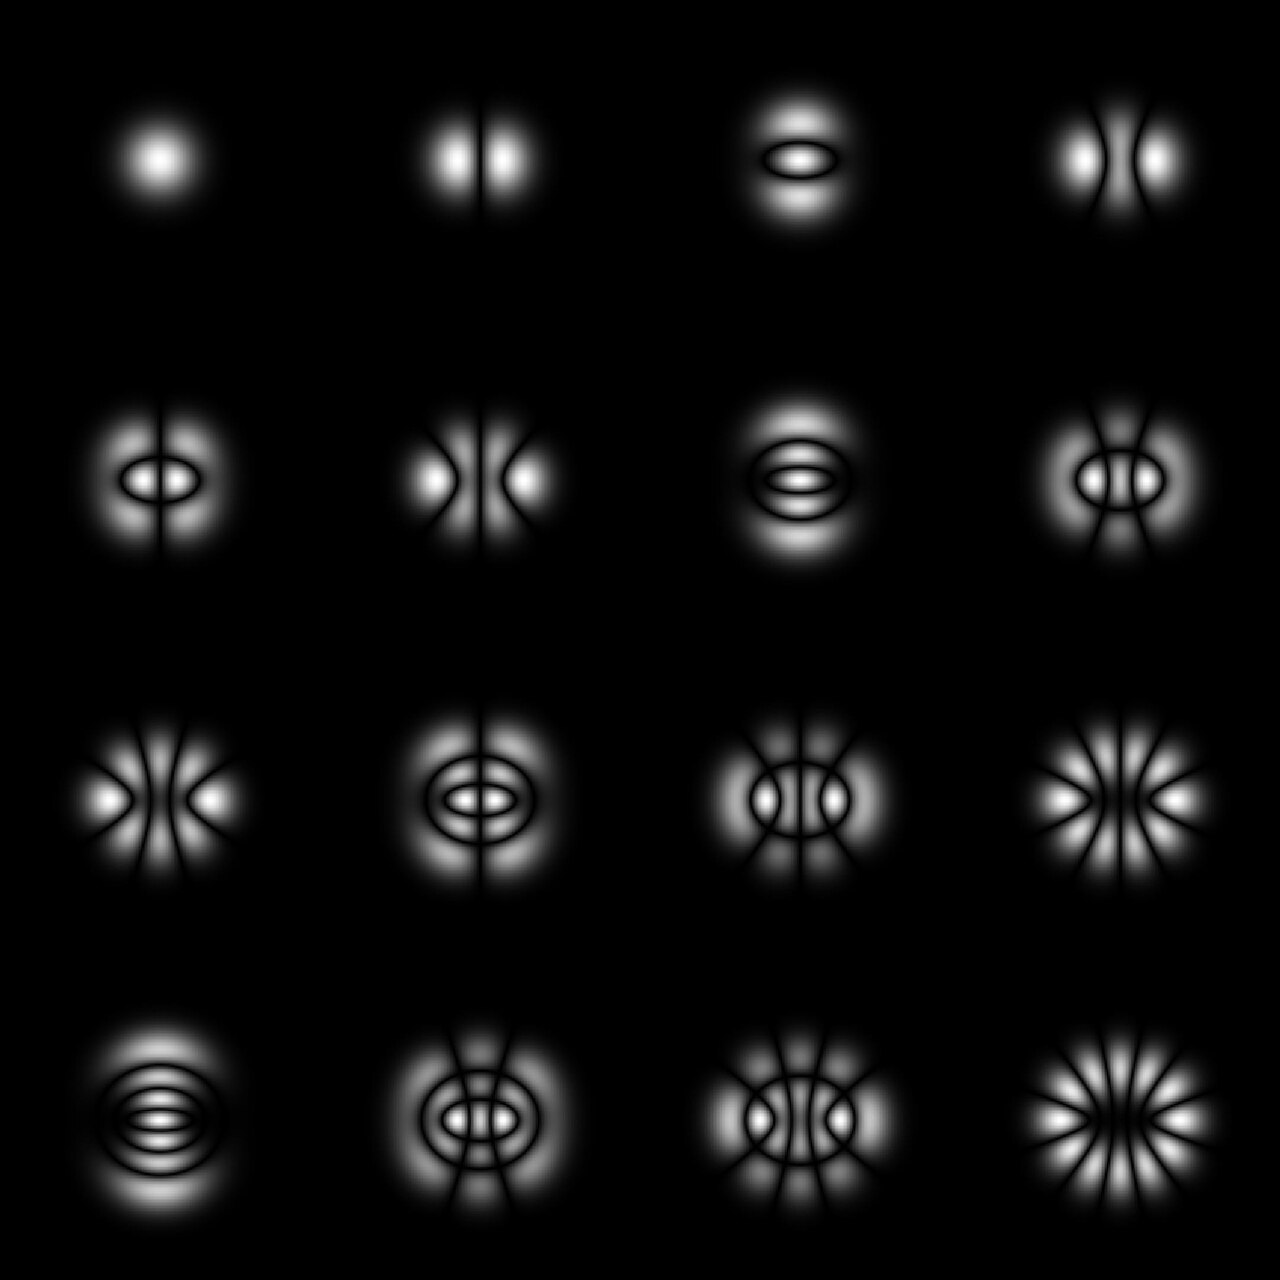
\includegraphics[width=0.35\linewidth]{images/APL1_8_Ince_Gaussian_Modes}
			\caption{最低阶偶数 Ince-Gaussian 模式的横向振幅分布(\cite{a})}
			\label{fig:apl18incegaussianmodes}
		\end{figure}
		
		\begin{figure}[htbp]
			\centering
			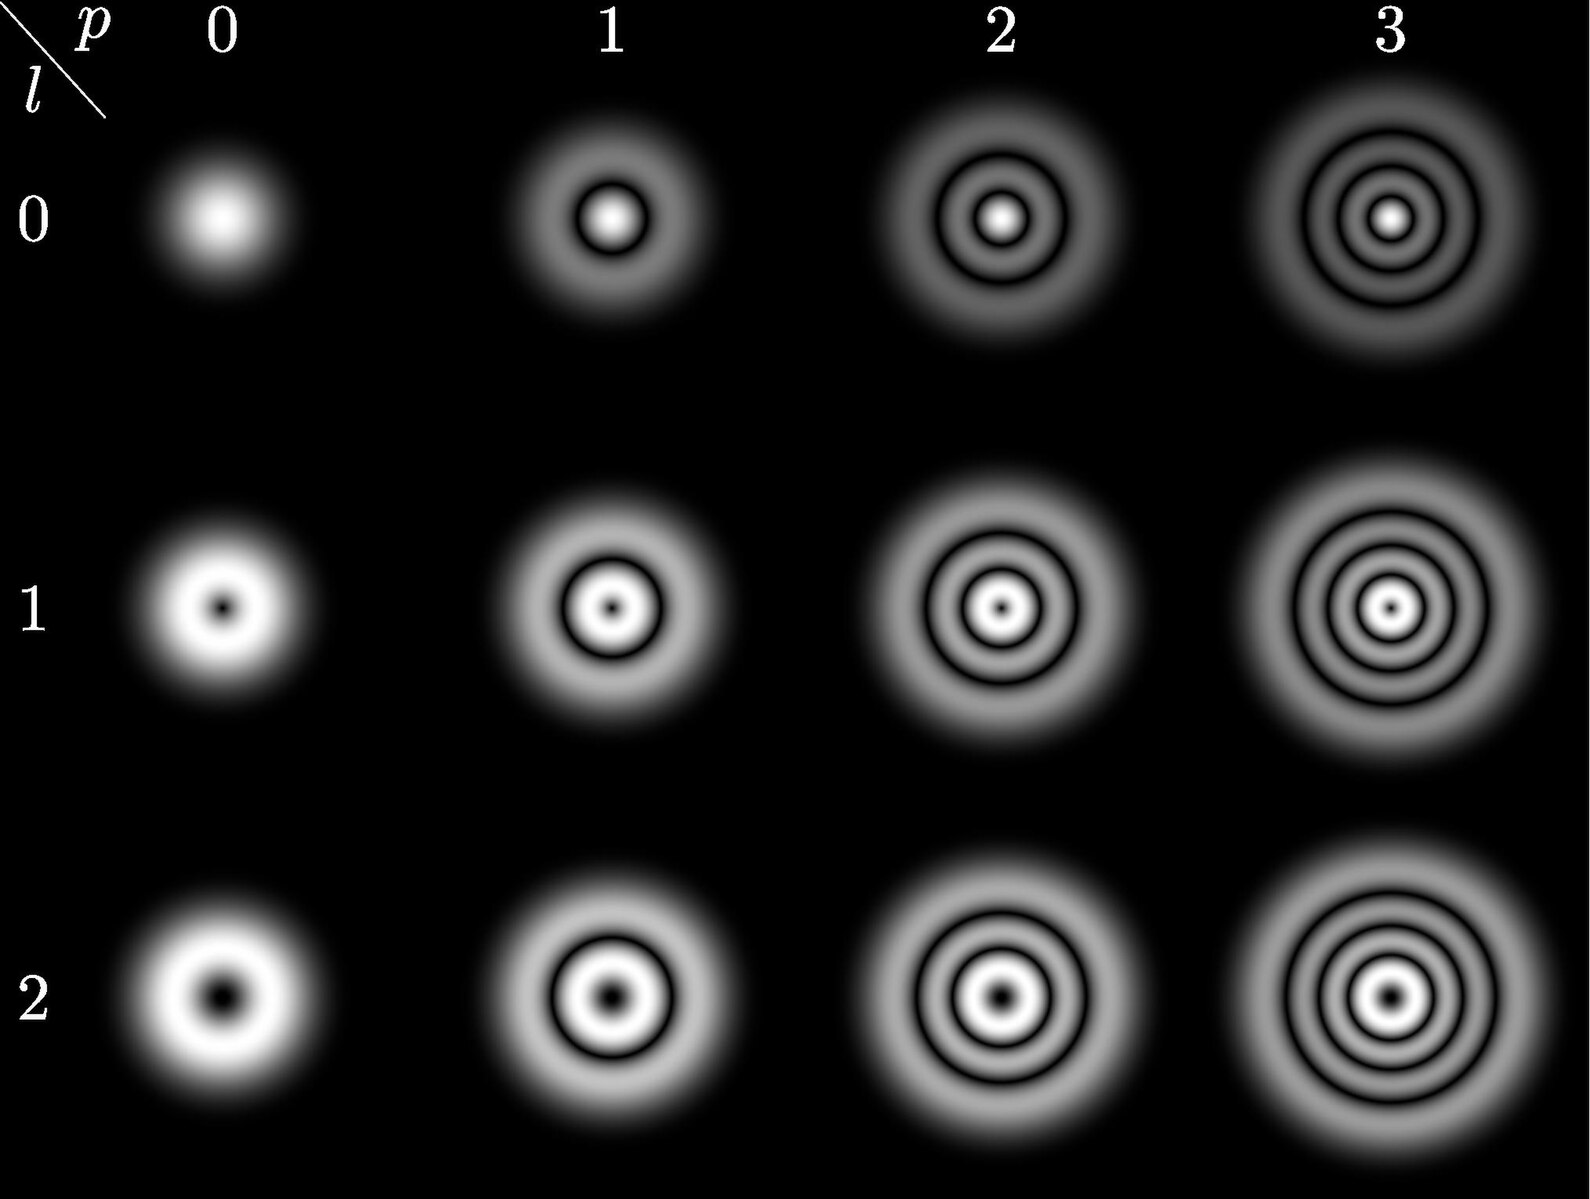
\includegraphics[width=0.35\linewidth]{images/APL1_8_Intensity_profiles_of_Laguerre-Gaussian_modes}
			\caption{前 12 个拉盖尔-高斯模式的强度分布(\cite{a})}
			\label{fig:apl18intensityprofilesoflaguerre-gaussianmodes}
		\end{figure}
		
		\begin{figure}[htbp]
			\centering
			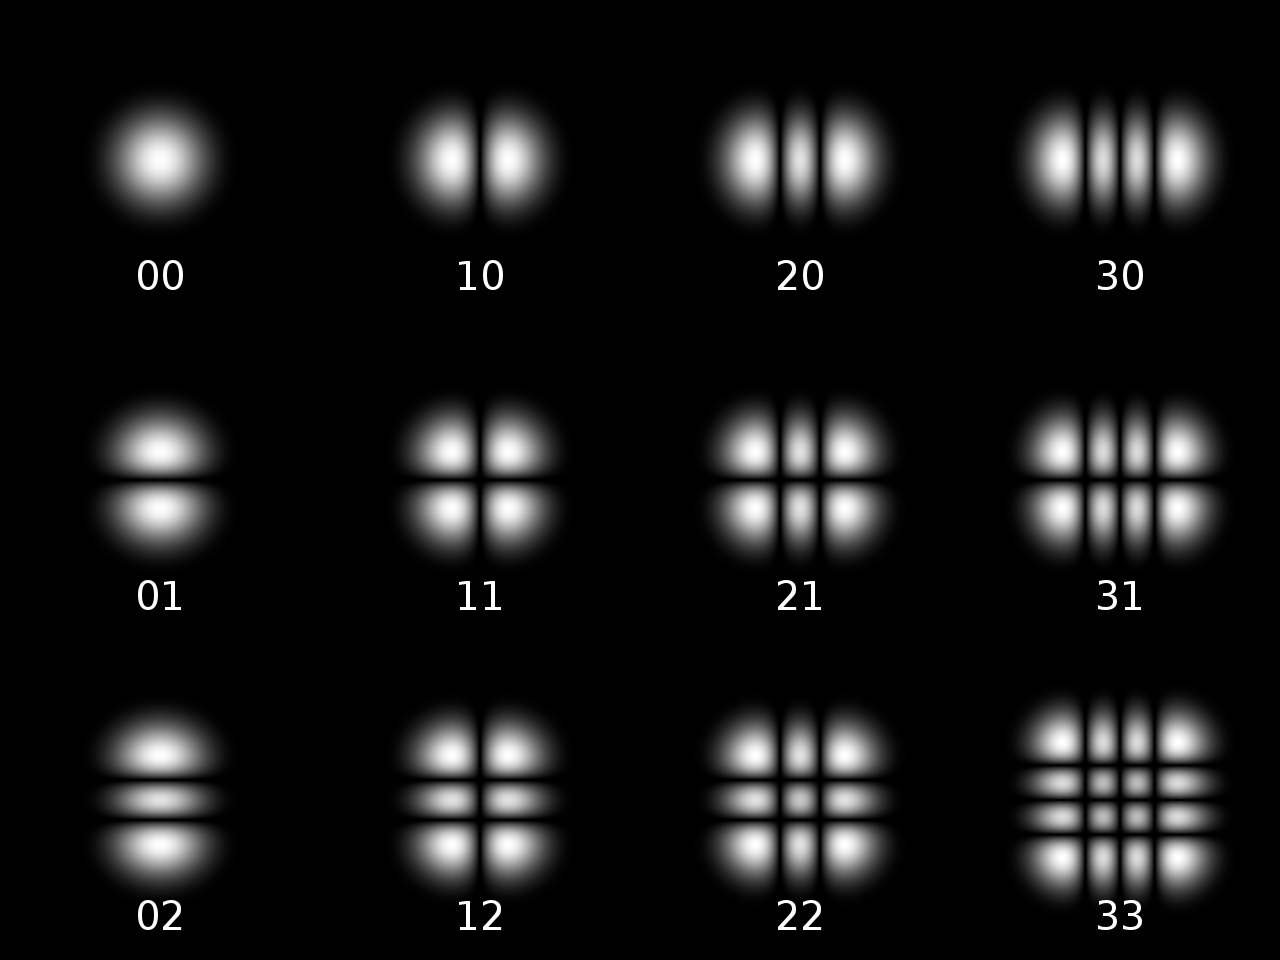
\includegraphics[width=0.37\linewidth]{images/APL1_8_Hermite-gaussian}
			\caption{十二个厄米-高斯模式(\cite{a})}
			\label{fig:apl18hermite-gaussian}
		\end{figure}
		
	\end{enumerate}
\end{enumerate}


%---------------------------------------------------------------------
% 实验前思考题
\subsection{Thinking Before Experiment}

% 思考题1
\begin{question}
	氦氖激光器产生激光的原理是什么?
	它在哪些领域有应用?
\end{question}
氦氖激光器的产生激光原理已经在\textbf{原理概述}部分有详细介绍了,以下是补充和总结。

氦氖(He-Ne)激光器是一种典型的气体激光器,通过氦(He)和氖(Ne)两种气体混合物的能级跃迁来实现激光的产生。其工作原理依赖于受激辐射,即当原子或分子被外界能量激发进入高能态时,在外部光子的作用下,它们会跃迁至低能态,并释放出与入射光子频率相同且相干的光子。该过程的能量关系可由公式 \(E = h \nu\) 表示,其中 \(E\) 为光子的能量,\(h\) 是普朗克常数(\(6.626 \times 10^{-34} \, \text{J·s}\)),\(\nu\) 是光子的频率。

在氦氖激光器中,主要依赖氦原子和氖原子的能级跃迁。氦原子在放电激发下被电子碰撞后,会进入亚稳态,如 \(2^3S_1\)。由于亚稳态寿命较长,氦原子能够将其能量通过共振能量转移给氖原子,使氖原子从基态跃迁至高能激发态。例如,氖原子可以从能级 \(E_1\) 跃迁至能级 \(E_3 = 20.66 \, \text{eV}\) 或 \(E_2 = 18.70 \, \text{eV}\),这两个能级之间的能量差对应于红色激光的波长。该激光的波长 \(\lambda\) 与频率的关系为:

\[
\lambda = \frac{c}{\nu} = \frac{hc}{E_3 - E_2}
\]

其中 \(c\) 为光速(\(3 \times 10^8 \, \text{m/s}\)),\(\lambda\) 为产生的红色激光波长,约为 632.8 nm。

氦氖激光器的工作机制通常用四能级系统来描述。首先,氦气体在高压放电中被电子碰撞,原子进入亚稳态;接着,氦原子通过共振将能量传递给氖原子,使其进入更高的能级。氖原子随后从高能态向低能态跃迁时,发射出红光激光。激光的产生依赖于粒子数反转,即系统中处于高能态的粒子数必须大于低能态的粒子数,满足 \(N_3 > N_2\) 的条件。这个过程可用速率方程描述:

\[
\frac{dN_3}{dt} = R - \frac{N_3}{\tau} - A_{32} N_3
\]

其中 \(R\) 是激发速率,\(\tau\) 是高能态的寿命,\(A_{32}\) 是自发辐射速率常数。在稳态条件下,即 \(\frac{dN_3}{dt} = 0\),高能态的粒子数 \(N_3\) 可表示为:

\[
N_3 = \frac{R \tau}{1 + A_{32} \tau}
\]

要实现稳定的激光输出,必须确保在高能态的粒子数大于低能态,这样受激辐射可以占主导地位。

氦氖激光器的另一个关键组件是谐振腔。谐振腔通常由两个反射镜组成,其中一个为全反射镜,另一个为部分透射镜。谐振腔的作用是使光子在腔内来回反射,从而经过多次放大后达到输出阈值。谐振腔的长度 \(L\) 必须满足激光的模条件:

\[
L = q \frac{\lambda}{2} \quad (q \in \mathbb{N})
\]

氦氖激光器由于其产生的激光具有高稳定性、单色性、低噪声和良好的方向性,因此在多个领域得到了广泛应用。首先,在科学研究与实验室中,氦氖激光器是光学实验和测量的重要工具。它常用于干涉测量,如迈克尔逊干涉仪和法布里-珀罗干涉仪,用于精确测量长度和折射率的变化。此外,它在全息摄影中凭借相干性拍摄和重现三维图像,并在散射光测量中分析颗粒物或分子的散射特性,例如动态光散射技术。氦氖激光器还被用作光学实验的波长或频率校准标准。 

在医疗与生命科学领域,氦氖激光器因其稳定的低功率输出和相对安全的红光波长(632.8 nm)而广泛应用于非侵入性治疗和诊断。例如,它在生物刺激治疗中被用来加速伤口愈合、减轻炎症和缓解疼痛,在眼科仪器中用于定位视网膜病变区域,并在牙科领域中用于口腔组织修复和牙龈炎症的处理。

氦氖激光器在工业与工程中也发挥着重要作用,尤其是在高精度对准、检测和加工领域。它被用于激光对准系统,提供精确的光轴指引,如隧道挖掘中的激光指向仪;在激光编码和检测中用于条形码扫描和表面缺陷检测;同时也在精密制造中监控加工过程中的位移变化和对准。

尽管氦氖激光器在现代通信中逐渐被半导体激光器所取代,但它仍在光通信教学和基础研究中占有一席之地。它常用于实验室演示光信号在光纤中的传输,并在测距仪和光学检测设备中作为系统校准光源。

此外,氦氖激光器在教育与培训中也是不可或缺的工具。在大学和科研机构的光学实验课程中,它被广泛用于激光干涉和衍射实验,帮助学生理解光波的相干性和干涉现象。此外,它还用于演示偏振器、分束器等光学仪器的工作原理。 

% 思考题2
\begin{question}
	请详细描述氦氖激光器的内部结构,包括哪些主要部件,并解释它们在激光产生过程中的作用。
\end{question}
在\textbf{原理概述}部分,我们对这个问题作了简要的讨论,可以参见\cref{fig:apl18typicalhenelasertubestructure}和\cref{fig:apl18laserstructure},以下我们对这个问题作进一步阐释。

氦氖激光器的内部结构包括多个关键部件,它们协同工作以实现激光的产生和稳定输出。这些部件主要包括放电管、气体混合物(氦气和氖气)、电极系统、谐振腔(反射镜系统)、激光输出窗以及冷却系统。放电管是激光器的核心结构,通常由玻璃或石英制成的细长管道构成,内部填充氦气和氖气的混合物,比例一般为氦:氖 ≈ 5:1。通过向放电管两端电极施加高电压,电子流穿过气体混合物,与氦原子碰撞,将其激发到高能态。这一过程是激光产生的初始步骤。

氦气和氖气的混合物在激光产生过程中扮演着重要角色。氦气的主要作用是吸收电子的动能并将能量通过共振转移给氖原子,使其进入高能态。这种共振能量转移基于氦的亚稳态(如 \(2^3S_1\))与氖原子的高能激发态之间的能级接近,从而实现高效的能量交换。氖原子在接收能量后从基态跃迁至高能态,并在随后向低能态跃迁时,通过受激辐射释放出红色激光。整个过程中,系统需要实现粒子数反转,即在某一时刻,高能态的氖原子数量多于低能态的,以确保受激辐射的增强。

电极系统位于放电管的两端,用于向气体混合物施加高电压,从而产生电子流。这些电子通过与氦原子碰撞,将其激发到亚稳态。电极系统的设计需要与放电效率相匹配,以确保电子流的稳定性,并提供足够的能量激发氦原子。

谐振腔系统是氦氖激光器的重要组成部分,通常由两个反射镜构成,分别为全反射镜和部分反射镜。全反射镜用于将所有反射回腔内,而部分反射镜则允许一部分光透射出来作为激光输出。谐振腔的作用是使光子在腔内反复反射,在每次反射过程中与更多的氖原子发生受激辐射相互作用,从而不断增强光子的数量和强度。谐振腔的长度 \(L\) 必须与激光波长匹配,以满足驻波条件 \(L = q \lambda / 2\)(其中 \(q\) 为正整数),以保证腔内的光波相干叠加。

激光输出窗位于部分反射镜的一侧,作为激光的出口。经过谐振腔内多次放大后的红光激光通过输出窗透射出来,波长为 632.8 nm。为了保证光束质量,输出窗的设计需要尽量减少光的衍射和散射。

由于放电过程会产生大量热量,氦氖激光器通常配备冷却系统来维持稳定的工作环境。常见的冷却方式包括自然空气冷却或风扇冷却,冷却系统的主要作用是防止温度升高导致气体压强变化,从而影响激光输出的稳定性。

氦氖激光器的工作过程始于电子流激发氦原子进入亚稳态,氦原子随后通过共振将能量传递给氖原子,使其进入高能激发态。当这些氖原子在光子的作用下从高能态向低能态跃迁时,会发生受激辐射,并释放出与入射光子频率相同且相干的光子。通过谐振腔内的多次反射和放大,最终从部分反射镜透射出稳定的激光。各部件的协调工作确保了氦氖激光器输出的激光具有高稳定性、优良的相干性和方向性。这些特性使氦氖激光器在科学研究、医疗、工业和教学等领域中得到了广泛的应用。

% 思考题3
\begin{question}
	什么是横模和纵模?
	它们对激光束的特性分别有什么影响?
\end{question}
关于这个问题,我们在\textbf{原理概述}部分给出了非常详尽的讨论,详见第2小节“\textbf{谐振腔的光场分布}”,此外,与之密切相关的\textbf{高斯光束}的理论分析可以参见第3小节第(4)部分“\textbf{高阶高斯模式}”。以下是一个常规性回答和总结。

在激光谐振腔中,光的传播可以按照不同的模式进行,这些模式根据光场的分布和传播方向不同,分为横模(Transverse Mode)和纵模(Longitudinal Mode)。横模描述的是光场在横截面上的分布,而纵模描述的是光场在光传播方向(轴向)上的分布。两者共同决定了激光束的形态、质量以及输出的光学特性。

横模(参见\cref{fig:apl18hermite-gaussian}、\cref{fig:apl18incegaussianmodes}和\cref{fig:apl18intensityprofilesoflaguerre-gaussianmodes})描述了垂直于激光束传播方向的光场分布。这些模式受到工作物质的横截面积和谐振腔镜面边界的限制,并因衍射而表现出不同的光强分布形式。常见的横模模式是高斯模式,其中基模为 TEM\(_{00}\) 模式。这种模式的光斑呈单一的高斯分布,中心光强最大,向外逐渐衰减。其光强分布可以表示为 \(I(x, y) = I_0 \exp(-2(x^2 + y^2)/w^2)\),其中 \(I_0\) 是中心的最大光强,\(w\) 是光束半径。除此之外,还有高阶横模,如 TEM\(_{01}\) 和 TEM\(_{10}\) 模式,它们的光斑中会出现多个亮斑。基模 TEM\(_{00}\) 模式的光束质量最佳,光束发散角最小,方向性强,而高阶横模的光束发散角较大,光束质量和准直性较差。

纵模描述了激光在谐振腔内沿传播方向的光场分布,对应于谐振腔内允许存在的离散频率模式。为了满足驻波条件,谐振腔的长度 \(L\) 必须为激光波长的整数倍的一半,即 \(L = q \lambda / 2\)。相邻纵模之间的频率间隔为 \(\Delta \nu = c / (2L)\),其中 \(c\) 是光速。由于不同纵模之间的频率存在微小差异,谐振腔内通常会同时存在多个纵模。

横模和纵模共同影响激光束的特性。横模主要影响光束的质量和发散角,基模 TEM\(_{00}\) 模式的光束中心光强高,具有良好的准直性和较小的发散角;而高阶横模的光斑中存在多个亮斑,发散角较大,光束在传播过程中易扩散。纵模的数量决定了激光的频谱宽度,纵模较少时激光的频率稳定、相干性好,适用于高精度测量;而多纵模激光器的频谱较宽,相干性较差,容易出现模式竞争,即增益较大的纵模抑制其他纵模的振荡,影响激光输出的稳定性。

激光器的实际输出模式通常是横模和纵模的叠加,既包含多种横模,也包含多个纵模。为了获得高质量的激光束输出,常需优化谐振腔设计,使激光器工作在单横模(如 TEM\(_{00}\) 模式)和单纵模状态下,这样能够确保激光具有优异的方向性、相干性和频率稳定性。横模和纵模的合理控制对于保证激光的性能和稳定性至关重要,是光学设计中的一个关键目标。

% 思考题4
\begin{question}
	什么是 q 参数?
	它在高斯光束的描述中起什么作用?
	如何通过 q 参数计算高斯光束的束腰半径和等相位面曲率半径?
\end{question}
关于高斯光束,我们在\textbf{原理概述}部分有着非常非常详细的讨论与分析,详见\textbf{第3小节“高斯光束”}。其中,\textbf{第(2)部分给出了关于“Complex Beam Parameter”}(也就是q参数)的详细理论,并于第(3)小节结合矩阵分析研究了\textbf{高斯光束的传播}。以下将是一个常规性回答与总结。

在高斯光束的描述中,q 参数是一种用来描述光束空间传播特性的复数参数,它综合了光束的发散、曲率和位置等信息,是高斯光束传播过程的核心参数。随着光束沿传播轴 \(z\) 传播,其光场可以用电场表达式表示为:\(E(r, z) = E_0 \frac{w_0}{w(z)} \exp\left(-\frac{r^2}{w^2(z)}\right) \exp\left(-ikz - ik\frac{r^2}{2R(z)} + i\psi(z)\right)\),其中 \(w(z)\) 是光束在 \(z\) 处的半径,\(R(z)\) 是等相位面的曲率半径,\(\psi(z)\) 是相位变化因子。这些参数随光束传播而不断变化,为了更好地描述光束在不同位置的状态,引入了 q 参数这一复数描述。

q 参数的定义为:\(\frac{1}{q(z)} = \frac{1}{R(z)} - i\frac{\lambda}{\pi w^2(z)}\)。其中 \(R(z)\) 是光束在 \(z\) 处的等相位面曲率半径,\(w(z)\) 是光束的半径,\(\lambda\) 是激光的波长。q 参数在光束传播中发挥了重要作用。它能综合地描述光束的半径变化与波前曲率的演化,并在光学系统中简化计算。q 参数尤其在使用 ABCD 矩阵法分析复杂光学系统中的光束传播时具有不可替代的作用,能够有效预测光束在透镜或其他光学元件后的状态。

通过 q 参数,可以计算出高斯光束的关键特性。光束的束腰半径 \(w_0\) 是光束在束腰处(即 \(z = 0\))的最小半径,束腰半径与瑞利长度 \(z_R\) 之间的关系为:\(z_R = \frac{\pi w_0^2}{\lambda}\)。瑞利长度表示光束在传播过程中保持准直的距离,越长的瑞利长度意味着光束的准直性能越好。此外,q 参数还能用于计算在某一位置 \(z\) 处的等相位面曲率半径 \(R(z)\),其表达式为:\(R(z) = z\left(1 + \frac{z_R^2}{z^2}\right)\)。在束腰处,即 \(z = 0\),\(R(0) \to \infty\),表示光束的波前为平面;而当 \(z \to \infty\) 时,\(R(z) \approx z\),说明光束的波前逐渐趋于球面。

q 参数不仅简化了高斯光束在自由空间中的传播描述,还在光学系统设计中得到了广泛应用。例如,通过 ABCD 矩阵法,可以用 q 参数轻松计算光束通过透镜后的传播情况。q 参数的引入让我们能够快速确定光束的半径、曲率及其传播特性,从而有效优化激光系统的性能。理解并掌握 q 参数的使用,对于实验与工程中的光学设计具有重要的意义,有助于更高效地设计和调整复杂的光学系统。